\chapter{Implementazione e testing}

A seguito di una trattazione teorica è seguita un'attività sperimentale atta a confrontare le euristiche 
studiate. La sperimentazione si è ispirata alla competizione ``DIMACS Implementation Challenge'' svoltasi 
nel $2000$, durante la quale sono state messe a confronto diverse euristiche sviluppate e implementate da 
ricercatori di ogni parte del mondo \cite{STSP}. Gli algoritmi sono stati testati sia su una serie di grafi 
generati casualmente, sia su una serie di grafi presenti in TSPLIB \cite{tsplib}.

\section{Scelte implementative}

L'implementazione delle euristiche e dei programmi di misurazione è stata svolta nel linguaggio \texttt{C++}: la 
scelta è dovuta alla flessibilità con cui il linguaggio permette l'astrazione pur mantenendo elevate prestazioni.
Di seguito verranno descritte, per ogni euristica, le strutture dati utilizzate e le scelte effettuate.

\subsection{Strutture dati comuni e ridefinizioni di tipo}

Le entità principali del problema sono il ``Tour'' e il ``Grafo''. Per quanto riguarda il Tour è stato 
deciso di utilizzare la classe \texttt{std::vector}, fornito dalla libreria standard del 
linguaggio. Il vantaggio principale di \texttt{std::vector} è il fatto di rappresentare un array 
ridimensionabile che fornisce sia l'accesso diretto ad un elemento (tramite indice), sia il ``push'' 
di un elemento in coda ad esso, entrambi con complessità $\mathcal{O}(1)$\footnote{Più precisamente, il 
\texttt{push\_back} ha complessità costante \textit{ammortizzata}: \texttt{std::vector} possiede una 
``capacità'' iniziale (un buffer interno allocato dinamicamente) e ogniqualvolta che un elemento deve essere 
``pushato'' ma il buffer è pieno, \texttt{std::vector} alloca un nuovo buffer di dimensione doppia; è facile 
notare come l'inserimento di $n$ elementi abbia quindi complessità $\mathcal{O}(n).$}. Queste performance sono 
quindi adatte per la gestione dei tour negli algoritmi ``tour construction''. Il Grafo in input,
invece, è stato rappresentato come matrice dei costi.

È stato fatto uso estensivo della keyword \texttt{typedef} per rendere più espressivo il codice: in questo modo,
semplici \texttt{double}, \texttt{int} o \texttt{std::vector<int>} vengono utilizzati come \texttt{Cost}, 
\texttt{Vertex} o \texttt{Tour}.

\subsection{Nearest Neighbor e Nearest Insertion}

È stato deciso di mantenere la semplicità concettuale delle due euristiche anche nell'implementazione: 
ad ogni passo vengono scansionati tutti i vertici alla ricerca del ``migliore'' libero, 
per poi aggiungerlo al tour parziale a seconda della politica di inserimento. Solo per quanto riguarda 
Nearest Insertion si è deciso di utilizzare una struttura dati di supporto, adatta agli inserimenti in 
posizioni arbitrarie della stessa: \texttt{std::list<>}. Anche in questo caso la classe viene 
offerta dalla libreria standard e rappresenta una lista concatenata. Il \texttt{typedef} utilizzato è 
\texttt{TourList}.

\subsection{Christofides}

L'algoritmo di Christofides richiede la costruzione di un Minimum Spanning Tree e di un Minimum Weight 
Matching. Per quanto riguarda l'MST si è deciso di utilizzare l'algoritmo di Prim, che è stato implementato 
senza l'uso di strutture dati particolari: la scelta è dovuta al fatto che, dovendo considerare solo grafi 
completi, l'utilizzo di Code con Priorità o algoritmi alternativi non avrebbe garantito prestazioni migliori. 
La costruzione del Minimum Weight Matching è stata invece semplificata: la strategia utilizzata è di tipo 
\textit{greedy} nel senso che vengono scansionati gli archi in ordine crescente di peso e viene scelto 
il primo incidente a due vertici non ancora aggiunti al matching. Infine, la ricerca del circuito 
euleriano è stata svolta ricorsivamente, modificando il classico algoritmo \textit{Depth First Search}: 
l'esistenza del circuito è assicurata dal Teorema 2.1.2 quindi è sufficiente visitare in profondità ogni arco non ancora 
visitato; dovendo effettuare inserimenti di vertici in posizioni arbitrarie del circuito che si sta 
costruendo, si è deciso di sfruttare \texttt{TourList}. Inoltre, avendo rappresentato gli archi non 
diretti del grafo come una coppia di archi diretti nei due versi opposti, sono state associate delle 
etichette in modo da riuscire a ricavarne una dall'altra. In questo modo è possibile ``visitare'' entrambi 
i versi di un arco che si sta per percorrere.\\

\begin{figure}[H]
    \centering
    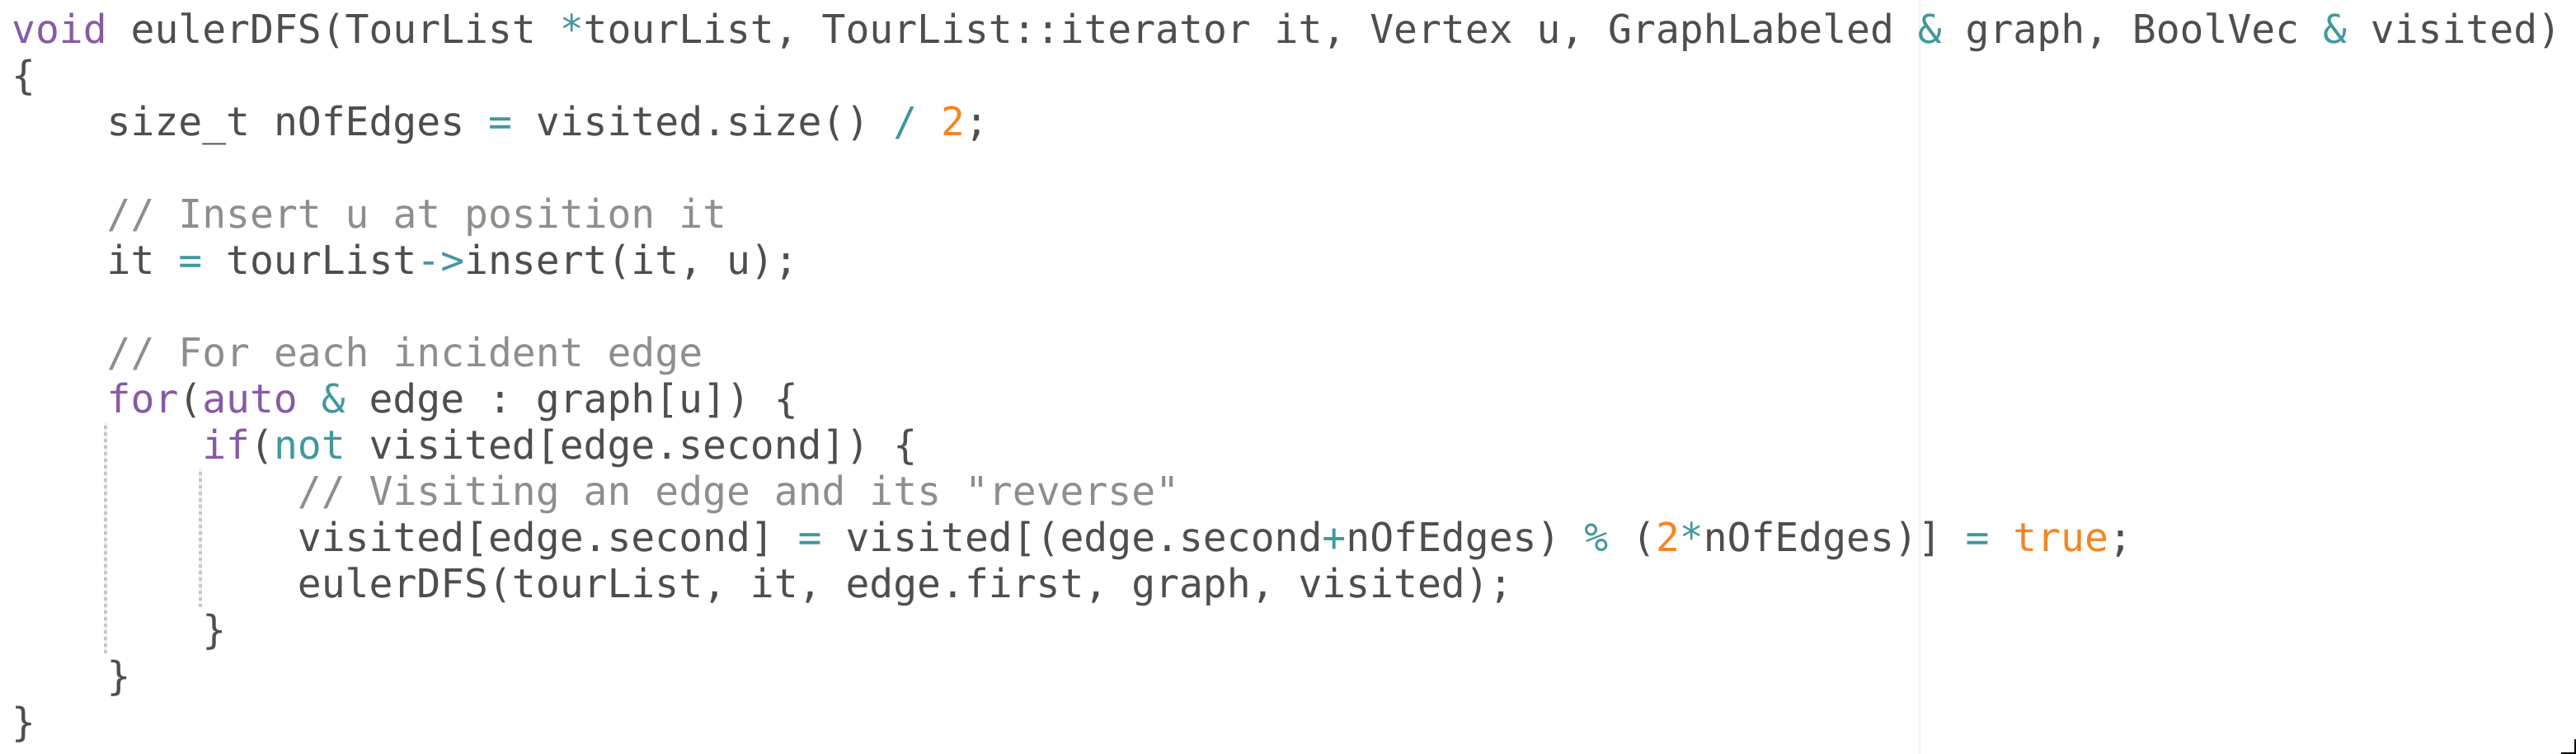
\includegraphics[width=450pt]{img/eulerDFS.png}
    \caption{Il codice per la ricerca del circuito euleriano.}
\end{figure}

\subsection{3-OPT}

L'implementazione scelta è quella descritta in \cite{3opt}. Si è mantenuta la scelta di utilizzare 
\texttt{std::vector} per rappresentare un Tour. Le MaxHeap, invece, sono state implementate sfruttando 
la classe \texttt{std::priority\_queue} fornita dalla libreria standard: è stato, tuttavia, definito il 
tipo di dato \texttt{HeapElement} dotato di operatore di confronto, così da rendere agevole l'utilizzo 
della coda. L'applicazione della mossa 3-OPT trovata viene fatta seguendo la costruzione a ``segmenti'' 
definita dallo \textit{schemda di reinserimento}: per evitare situazioni limite (segmenti che sono a cavallo 
tra inizio e fine del tour) è stato deciso di raddoppiare il circuito, così da ``simulare'', attraverso il 
\texttt{vector}, la ciclicità. È stata utilizzata la funzione \texttt{std::reverse()} per capovolgere i 
segmenti che vengono percorsi in senso antiorario: il tour viene quindi costruito accodando i diversi 
segmenti con l'orientamento definito dallo schema.
\ \\

\begin{figure}[H]
    \centering
    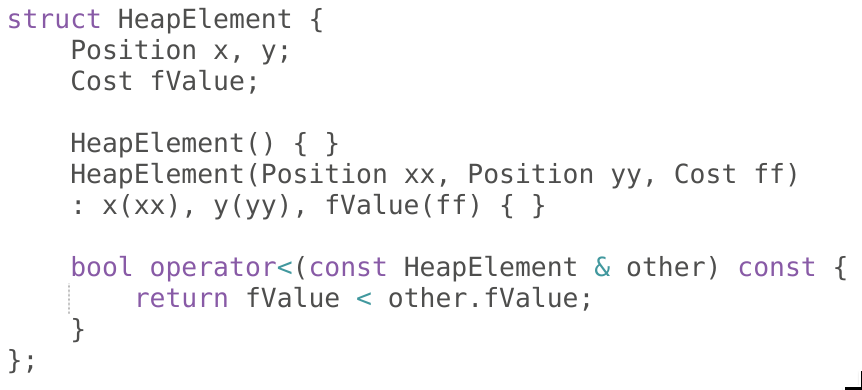
\includegraphics[width=250pt]{img/HeapElement.png}
    \caption{Il tipo di dato HeapElement.}
\end{figure}
\ \\
Sono state sviluppate tre varianti di 3-OPT:
\begin{description}
    \item[\texttt{random3opt}:] il tour iniziale viene generato casualmente.
    \item[\texttt{christofides3opt}:] il tour iniziale viene generato con l'algoritmo \texttt{CHR}.
    \item[\texttt{reiterated3opt}:] inizialmente il tour viene generato con \texttt{CHR}; quando viene 
            trovato un minimo locale, il tour viene ``perturbato'' scambiando casualmente alcuni vertici.
            La procedura quindi viene eseguita a partire da questo tour perturbato; la scelta di quanti 
            vertici scambiare e di quante volte reiterare viene decisa parametricamente: in particolare,
            viene mantenuto un parametro \texttt{maxIteration} che viene incrementato ogni volta che 
            viene prodotto un minimo locale migliore dei precedenti e la procedura termina quando vengono 
            eseguite \texttt{maxIteration} iterazioni.   
\end{description}

\subsection{Lin-Kernighan-Helsgaun (\texttt{LKH})}

A causa della complessità implementativa di questo algoritmo è stato deciso di seguire l'approccio 
descritto in \cite{LKH}: il tour viene rappresentato come una lista concatenata di elementi di tipo 
\texttt{LKHNode}. Come nel caso di Christofides, si è deciso di semplificare l'algoritmo rispetto a quello 
ufficiale: il tour iniziale non viene generato con l'euristica costruttiva di 
Helsgaun ma con \texttt{CHR}; questa scelta viene giustificata in \cite{LKH}. Un'altra scelta 
discordante con l'algoritmo di Helsgaun è nelle ``mosse base'': in \cite{LKH} vengono utilizzate mosse 
sequenziali 5-OPT; si è deciso invece di utilizzare mosse sequenziali 3-OPT per favorire la leggibilità 
del codice pur mantenendo la struttura originale dell'algoritmo. 

La procedura, come descritta da Helsgaun, costruisce gli \textit{insiemi dei candidati} 
basandosi sulla nozione di $\alpha$-nearness migliorata. Questa viene calcolata da un 
M$1$T del grafo perturbato, massimizzando $\pi$ con il metodo del subgradiente (nel codice, \texttt{ascent}).
\ \\

\begin{figure}[H]
    \centering
    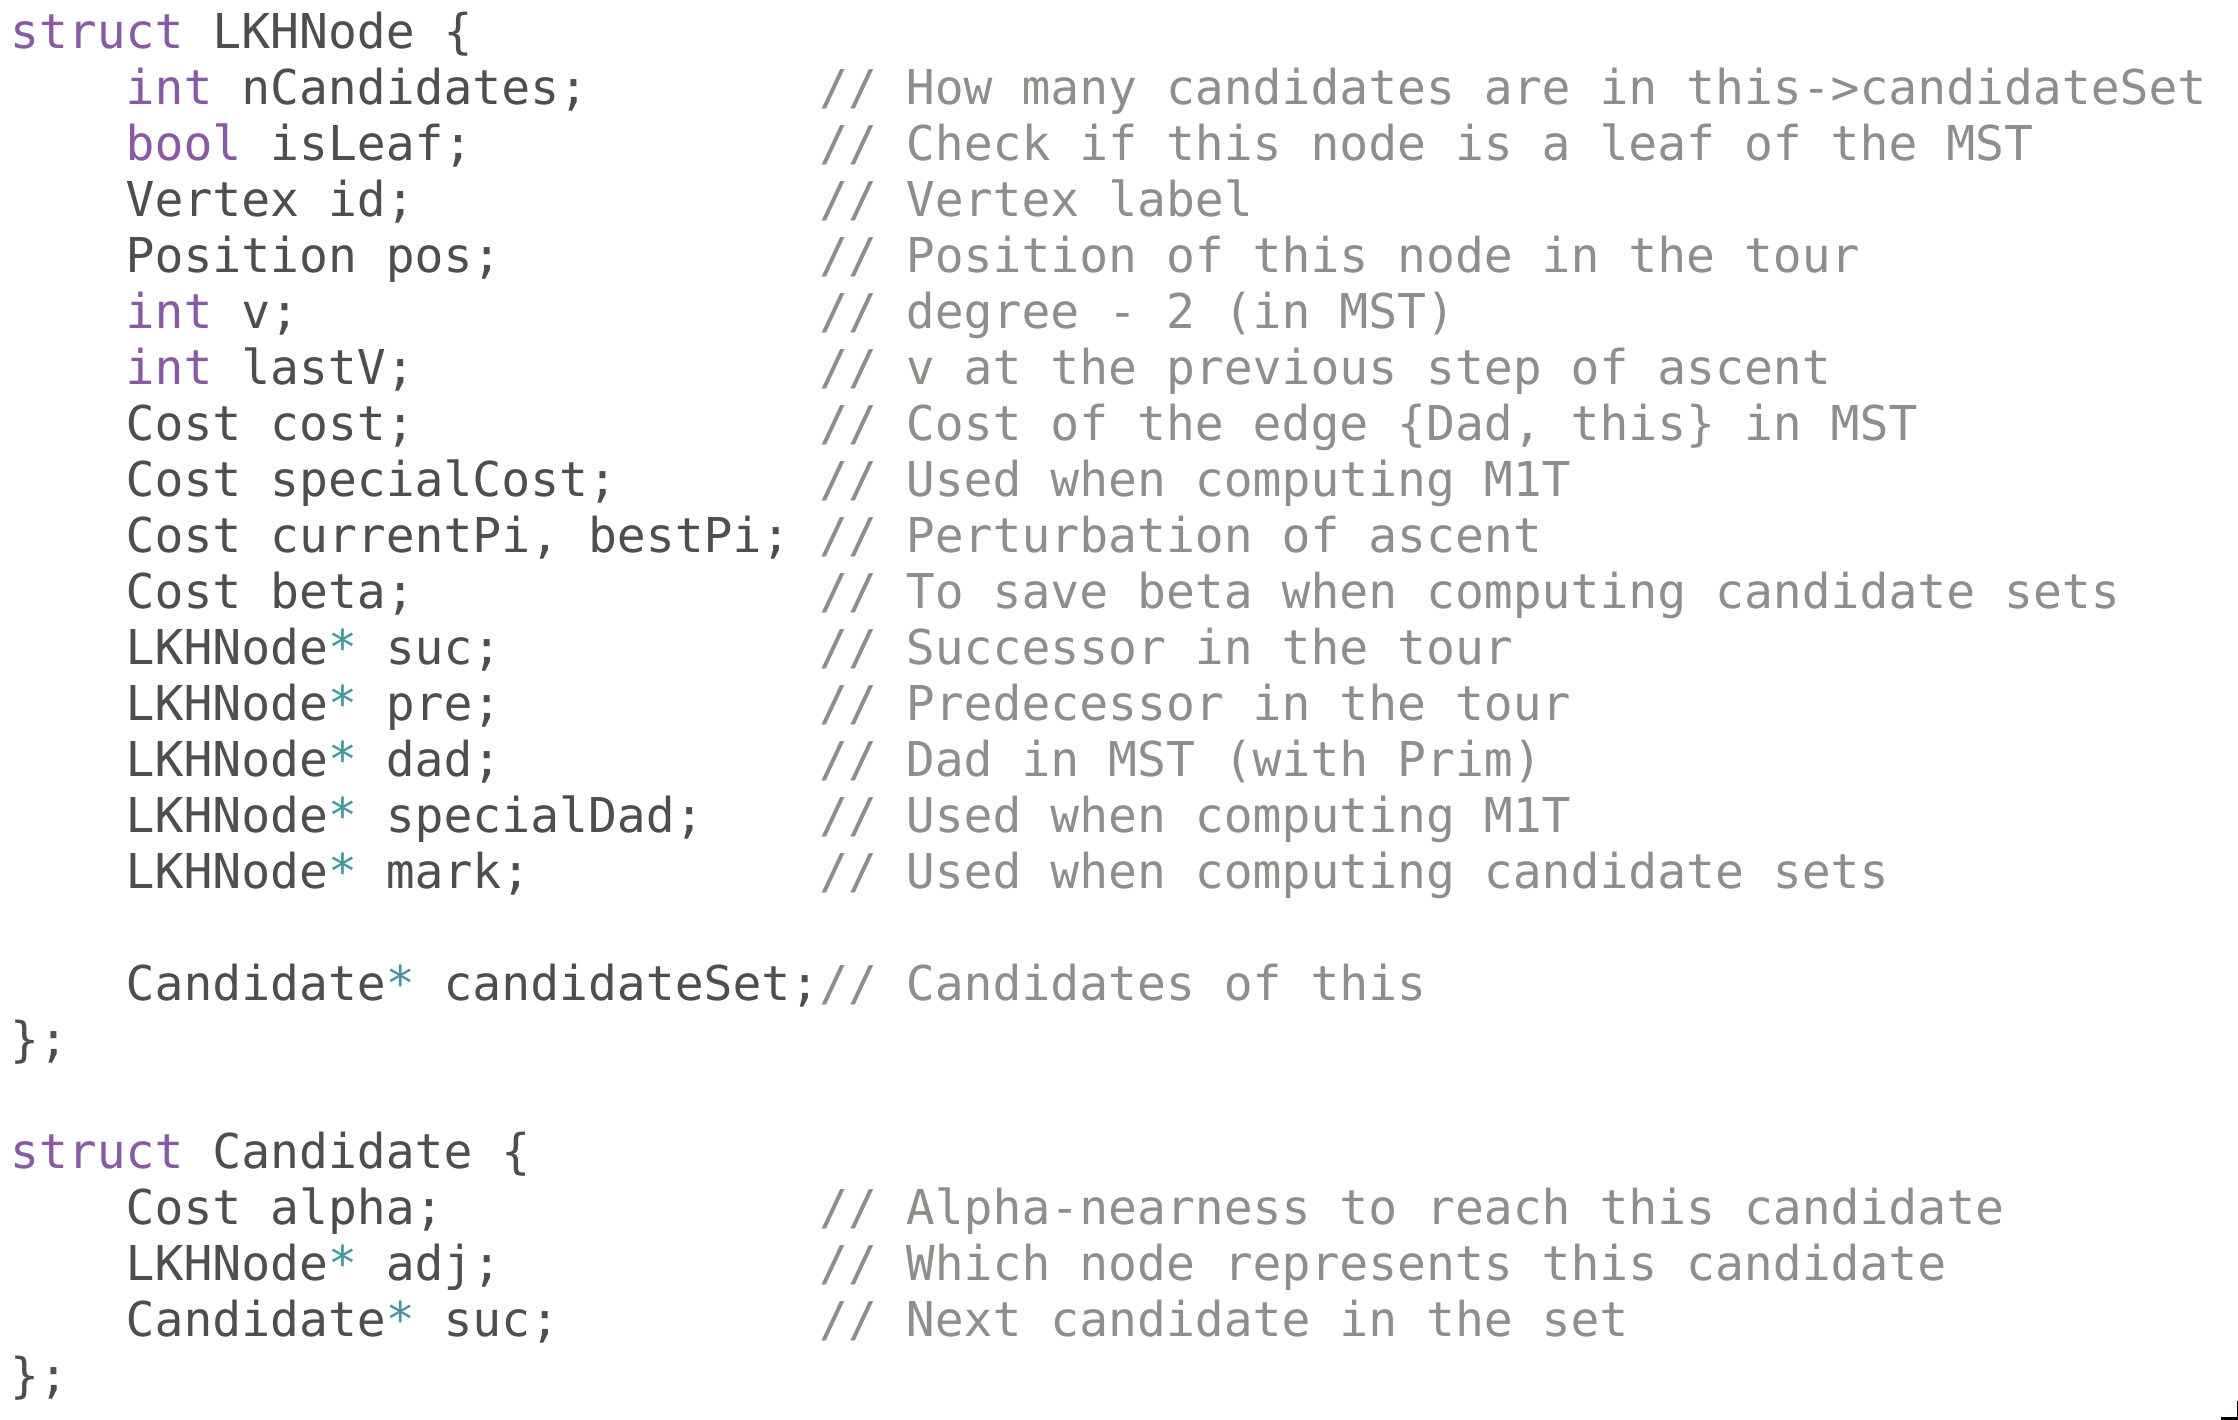
\includegraphics[width=350pt]{img/LKHNode.png}
    \caption{Tipi di dato \texttt{LKHNode} e \texttt{Candidate}.}
\end{figure}


Una volta generati i candidati vengono effettuate \texttt{maxRuns} iterazioni: ad ogni iterazione viene generato 
un tour con \texttt{CHR} e per \texttt{maxTrials} iterazioni viene eseguito \texttt{linKernighan} su tale tour. Al termine 
di ogni ``trial'', se si è trovato un tour migliore dei precedenti, i candidati vengono modificati inserendo 
gli archi del tour migliorato. Al termine di ogni ``run'', viene salvato il migliore dei tour rispetto alle run 
precedenti.

\begin{figure}[H]
    \centering
    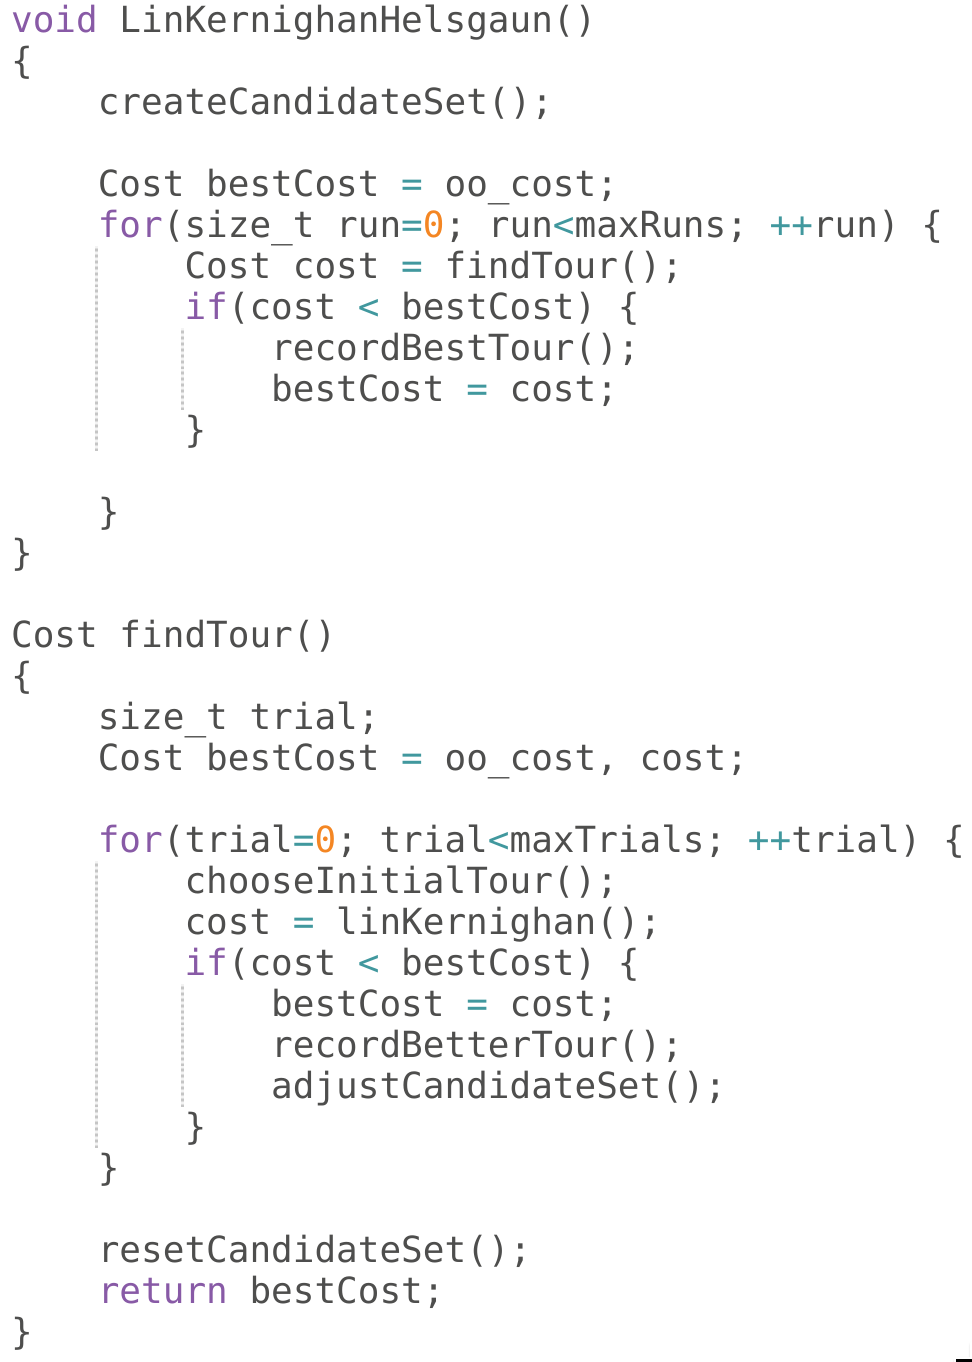
\includegraphics[width=225pt]{img/LKHProcedure.png}
    \caption{Lo ``scheletro'' della procedura.}
\end{figure}

Ogni volta che viene trovata una mossa 2-OPT o 3-OPT che porti ad un tour meno pesante, questa viene applicata.
Se, invece, non esistono tali mosse, viene applicata la mossa 3-OPT più vantaggiosa e la procedura si ripete 
cercando di ``rompere'' l'ultimo arco aggiunto dalla 3-OPT della mossa precedente; viene inoltre mantenuta 
una pila delle mosse effettuate: se si ottiene un miglioramento del tour, tale pila viene svuotata; altrimenti, 
la pila viene utilizzata per ripristinare il tour precedente (quello che potremmo definire un ``undo'').

Sono state poi analizzate le mosse 3-OPT sequenziali e si è ricavata una procedura per scomporre tali mosse in 
al più tre 2-OPT sequenziali, così da semplificare ulteriormente il codice.

\begin{figure}[H]
    \centering
    \begin{subfigure}{\linewidth}
        \centering
        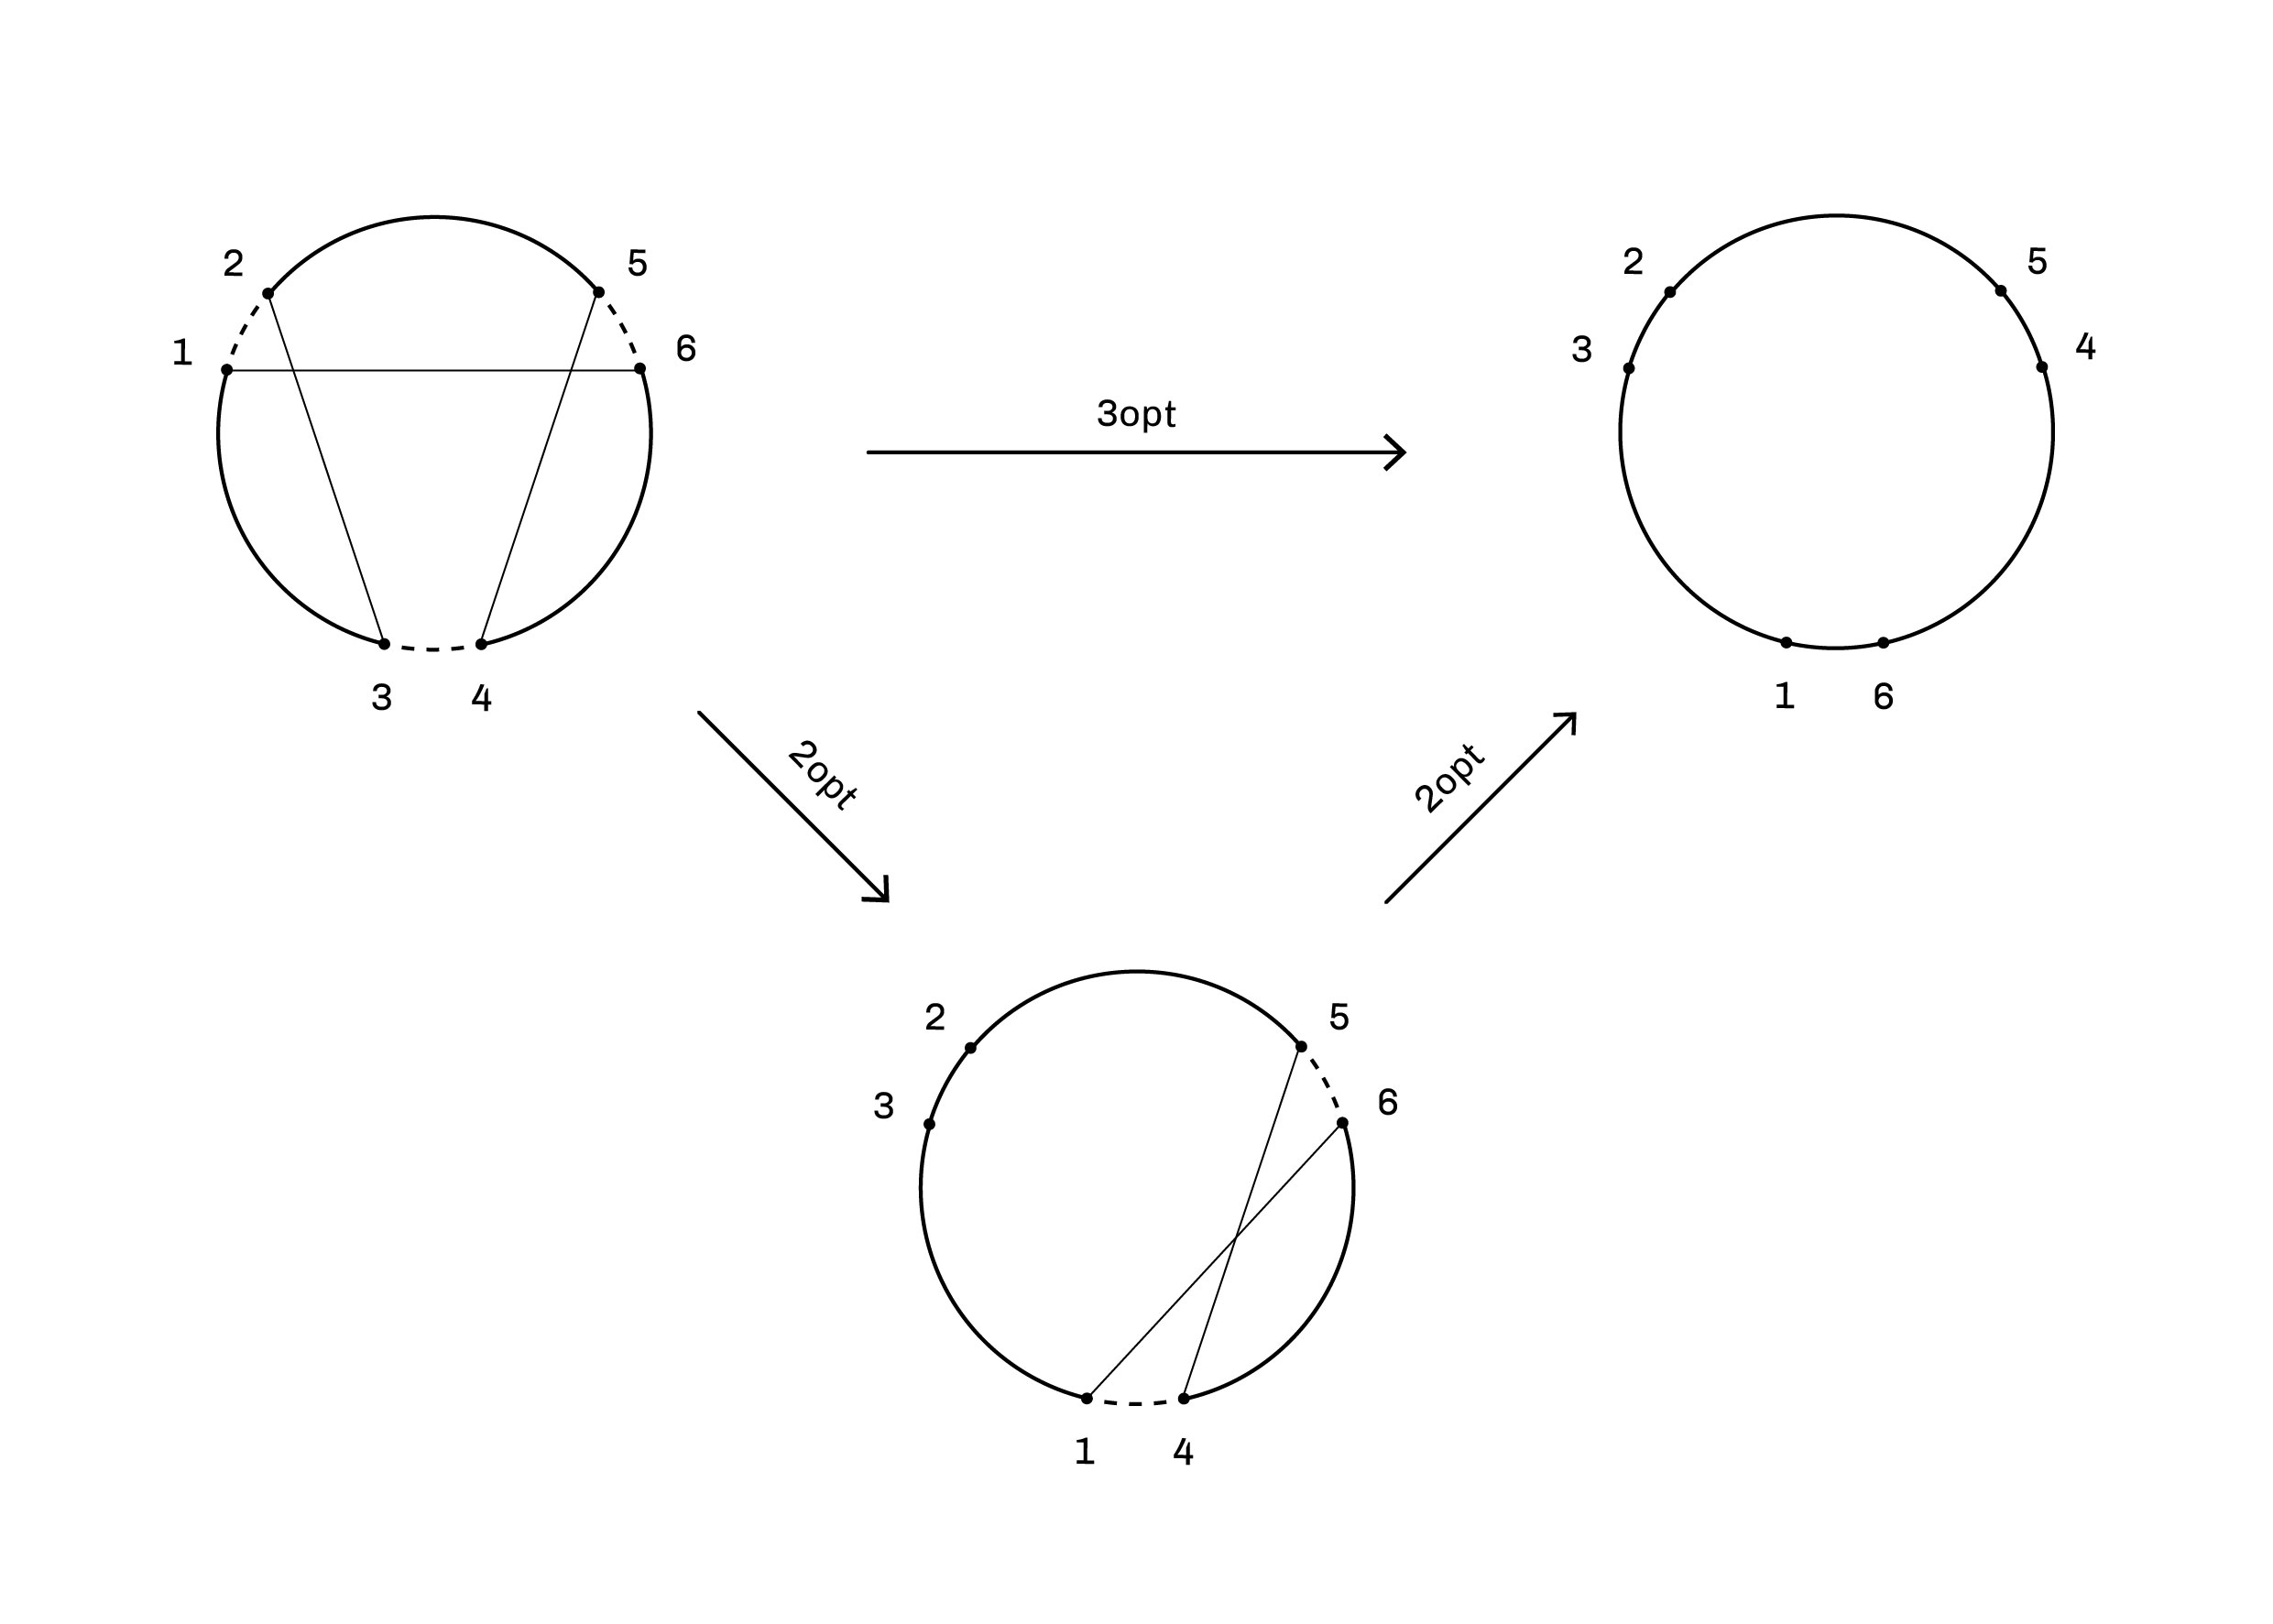
\includegraphics[width=340pt]{img/schemaH.jpg}
        \caption{}
    \end{subfigure}
    \begin{subfigure}{\linewidth}
        \centering
        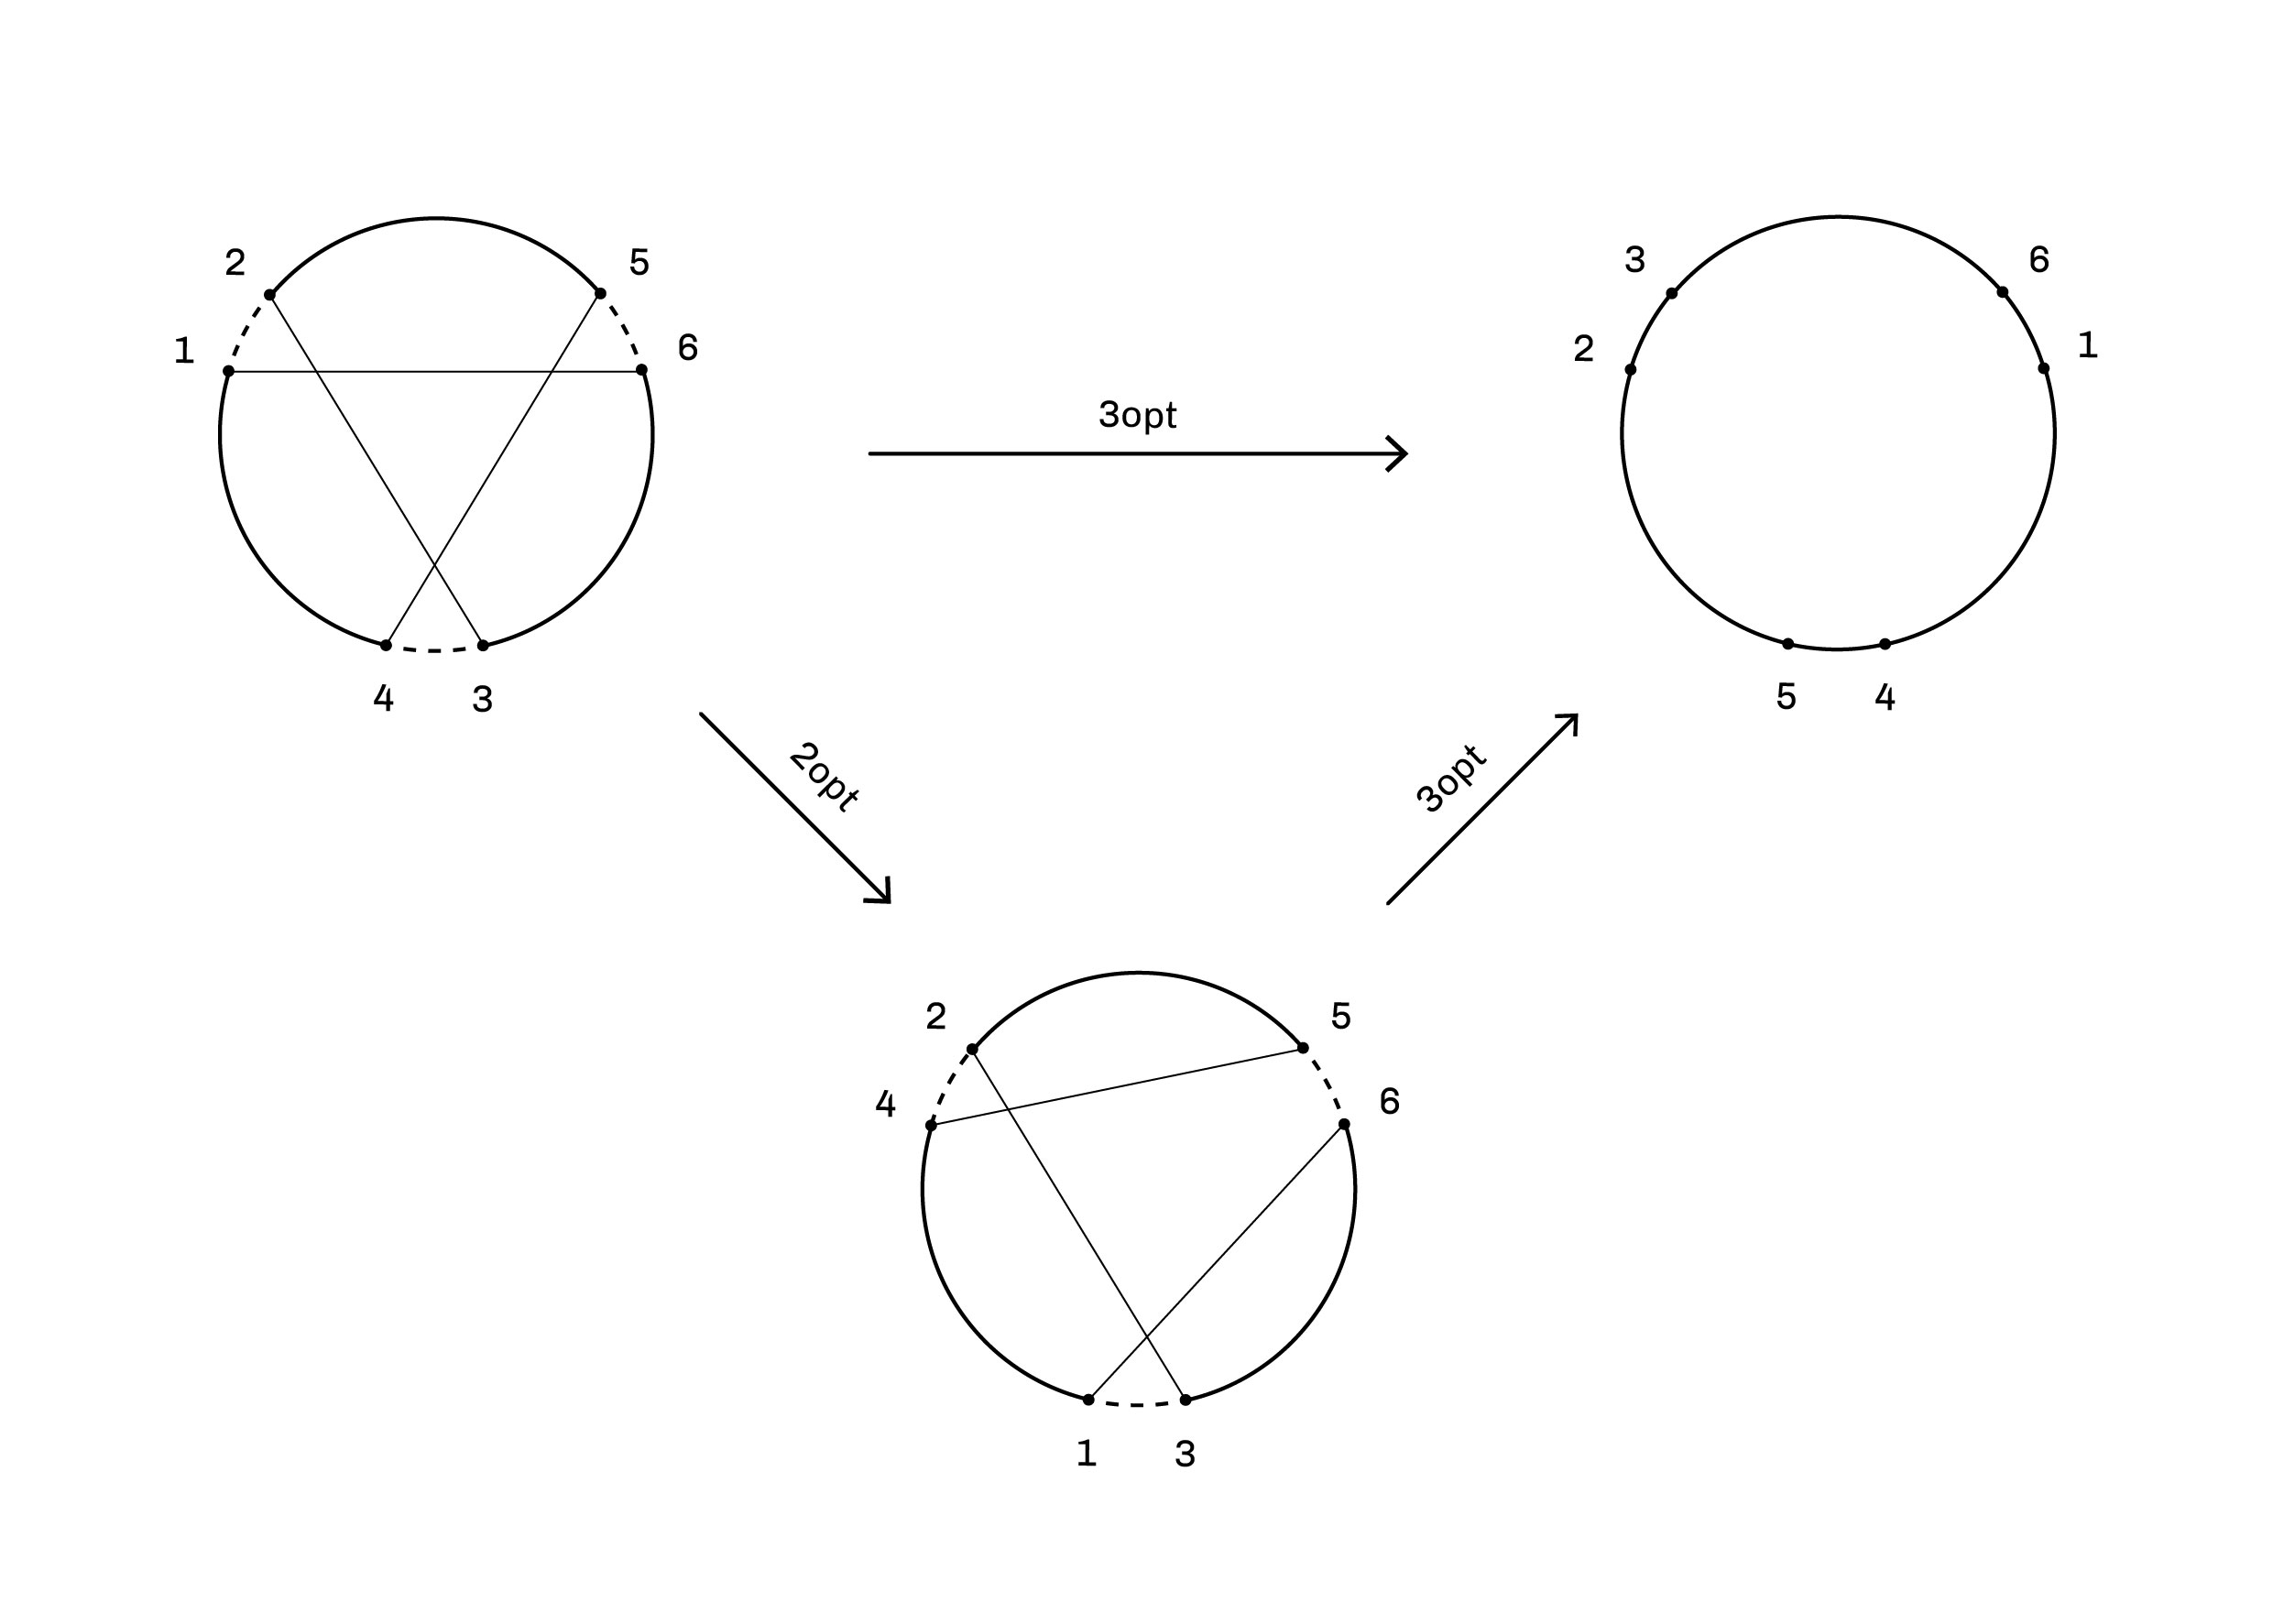
\includegraphics[width=340pt]{img/schemaXX.jpg}
        \caption{}
    \end{subfigure}
    \caption{Vengono descritte le trasformazioni che permettono di effettuare una 3-OPT come combinazione 
            di 2-OPT. Vi sono quattro tipi di 3-OPT sequenziali che emergono dall'algoritmo. Tre di 
            questi sono simmetrici per rotazione al caso (a): questo può essere simulato con due 2-OPT. 
            Notiamo poi che il quarto tipo, il caso (b), è riconducibile al caso (a) mediante un'applicazione di 2-OPT.}
\end{figure}

\section{Soggetto della misura}

Durante la fase sperimentale ci siamo focalizzati su due aspetti fondamentali di un'euristica: tempo di esecuzione 
e rapporto (empirico) di approssimazione. Sono stati utilizzati due tipi di di campione: 
\begin{itemize}
    \item Un insieme di grafi completi di $n \in \{100, 200, 300, 500, 1000, 2000, 3000, 5000\}$ nodi, con pesi 
            distribuiti uniformemente nell'intervallo $\big[1,n^2\big]\cap \mathbb{N}$.
    
    \item Un insieme di grafi presenti in \texttt{TSPLIB}; sono stati scelti \texttt{a280}, 
            \texttt{pr439}, \texttt{u1060}, \texttt{vm1748}, \texttt{pr2392}.
\end{itemize}

Inoltre, per \texttt{3-OPT} con reiterazione sono stati studiati tempo di esecuzione e qualità dell'approssimazione al variare 
di \texttt{maxExchanges}, mentre per \texttt{LKH} sono stati studiati tempo di esecuzione e qualità dell'approssimazione 
al variare di \texttt{maxCandidates}. Entrambi gli studi sono stati svolti su un campione di cinque grafi generati 
casualmente di $n=1000$ nodi.

La qualità dell'approssimazione è l'errore relativo del costo del tour trovato dall'euristica rispetto al costo ottimo,
$$\epsilon = \frac{C_{eur}-C_{opt}}{C_{opt}}$$

Per le istanze scelte di \texttt{TSPLIB} l'ottimo è noto; per i grafi generati casualmente si è cercato di approssimare 
l'ottimo con la bound di Held-Karp calcolata attraverso \texttt{ascent}. Sfortunatamente, la differenza percentuale tra 
le bound approssimate e i costi dei tour superavano, in alcuni casi, i $5000$ punti: l'ipotesi è che la distribuzione 
uniforme dei costi degli archi abbia sensibilmente abbassato la bound di Held-Karp rispetto al tour ottimo. In mancanza 
di evidenze sperimentali che ci permettessero di sfruttare efficacemente il valore calcolato da \texttt{ascent} si è 
deciso di non assegnare un errore ai costi dei tour nei grafi casuali.

\section{Modalità di misurazione del tempo di esecuzione}

La macchina su cui sono stati svolti i test è un Dell XPS-13 9370 con cpu Intel Core i5-82500U, 4 core (8 thread) da 
1.60GHz (3.40GHz in Turbo Boost) e 8GB di memoria Ram.

Per evitare di incorrere in risultati non affidabili la misurazione del tempo di esecuzione è stata svolta 
seguendo la procedura descritta in \cite{Poli}. È stato definito un'intervallo di confidenza all'$(1-\alpha)$ 
per $\alpha=0.05$ e, per ogni dimensione $n$, è stato generato un campione di cinque grafi di $n$ nodi: per quanto 
riguarda i grafi di \texttt{TSPLIB} tale campione è stato costruito con cinque copie dello stesso grafo.

\section{Randomness}

La casualità è uno strumento fondamentale nell'Informatica: essa permette di ottenere algoritmi più efficienti, 
strutture dati più robuste e simulazioni più realistiche. Ognuna delle euristiche descritte utilizza, in misura 
diversa, la \textit{randomness}. Non solo, anche la procedura di misurazione descritta precedentemente utilizza 
la randomness per la generazione dei campioni. È quindi necessario un algoritmo che approssimi 
sufficientemente bene la casualità: a differenza del linguaggio \texttt{C} e altri, il \texttt{C++} mette a 
disposizione la libreria \texttt{<random>} per gestire distribuzioni e generatori di numeri (pseudo)casuali. 
Tra i generatori lineari congruenziali è presente un'implementazione del prng Park-Miller (che viene 
utilizzato anche in \cite{Poli}). È stato quindi scelto tale generatore per effettuare ogni operazione che 
coinvolgesse la randomness.

\section{Risultati e confronti}

\subsection{Tabelle dei risultati}

Vengono di seguito presentati i risultati degli esperimenti effettuati. I tempi sono espressi in 
secondi, ``Errore (\%)'' è $\epsilon\cdot{}100$, ``Diff T (\%)'' e ``Diff C (\%)'' sono le differenze 
percentuali rispetto al valore di riferimenti: nel caso di \texttt{RL3O} è di $10$ scambi, nel caso di 
\texttt{LKH} è di $30$ candidati. In questa sottosezione ci limitiamo a fornire le tabelle dei dati; 
questi verranno confrontati e commentati nella successiva.
\ \\
\ \\
\ \\

\begin{figure}[H]
    \centering
    \begin{subfigure}{\linewidth}
        \centering
        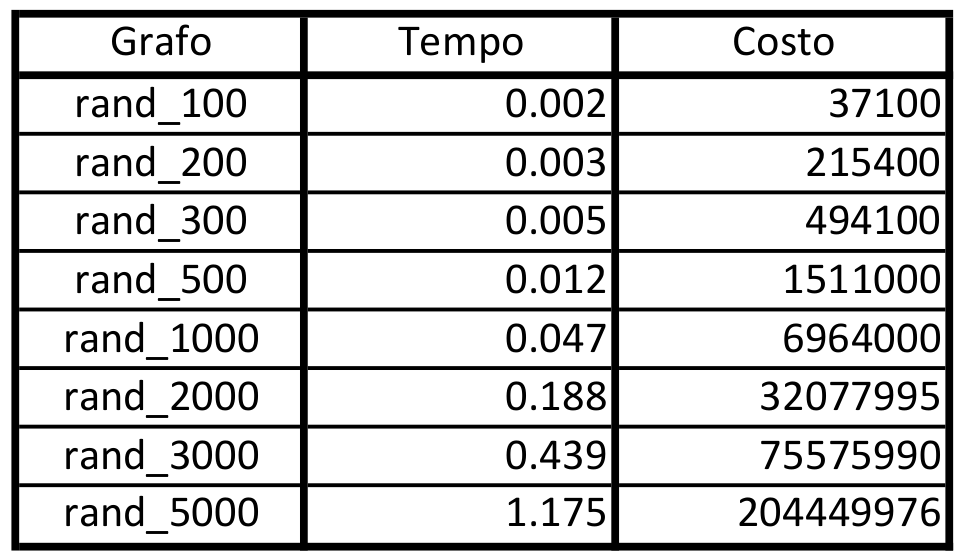
\includegraphics[width=200pt]{img/NNrandom.png}
        \caption*{Su grafi generati casualmente.}
    \end{subfigure}
    \ \\
    \ \\
    \ \\
    \ \\
    \begin{subfigure}{\linewidth}
        \centering
        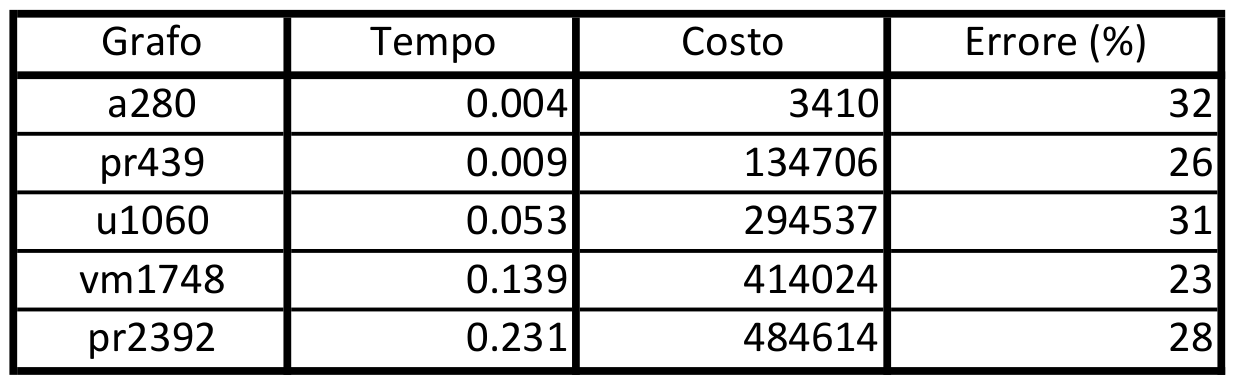
\includegraphics[width=300pt]{img/NNtsplib.png}
        \caption*{Su grafi di \texttt{TSPLIB}.}
    \end{subfigure}
    \caption{Risultati \texttt{NN}.}
\end{figure}
\ \\
\ \\

\begin{figure}[H]
    \centering
    \begin{subfigure}{\linewidth}
        \centering
        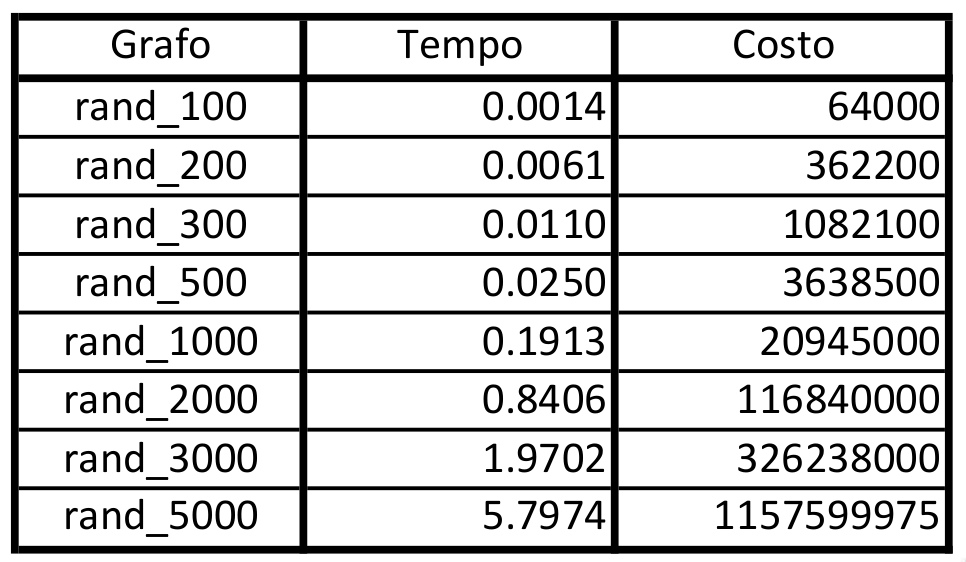
\includegraphics[width=200pt]{img/NIrandom.png}
        \caption*{Su grafi generati casualmente.}
    \end{subfigure}
    \ \\
    \ \\
    \ \\
    \ \\
    \begin{subfigure}{\linewidth}
        \centering
        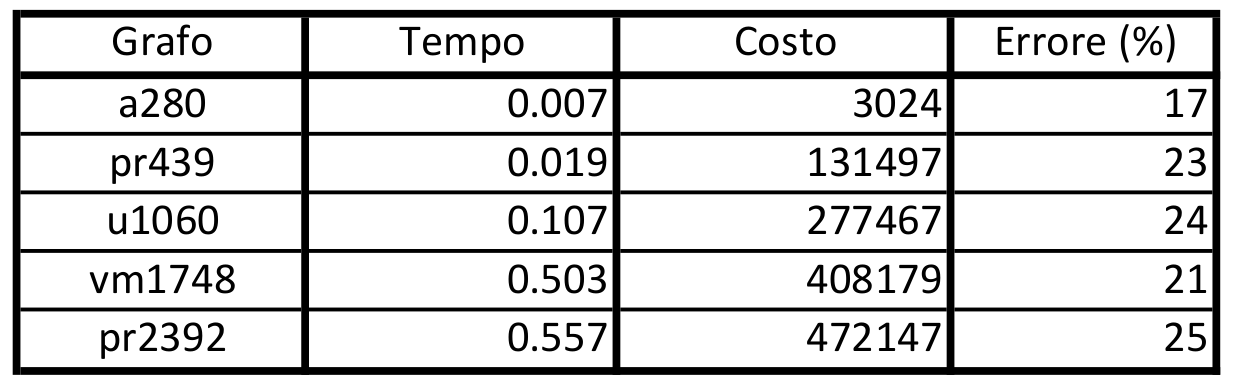
\includegraphics[width=300pt]{img/NItsplib.png}
        \caption*{Su grafi di \texttt{TSPLIB}.}
    \end{subfigure}
    \caption{Risultati \texttt{NI}.}
\end{figure}
\ \\
\ \\

\begin{figure}[H]
    \centering
    \begin{subfigure}{\linewidth}
        \centering
        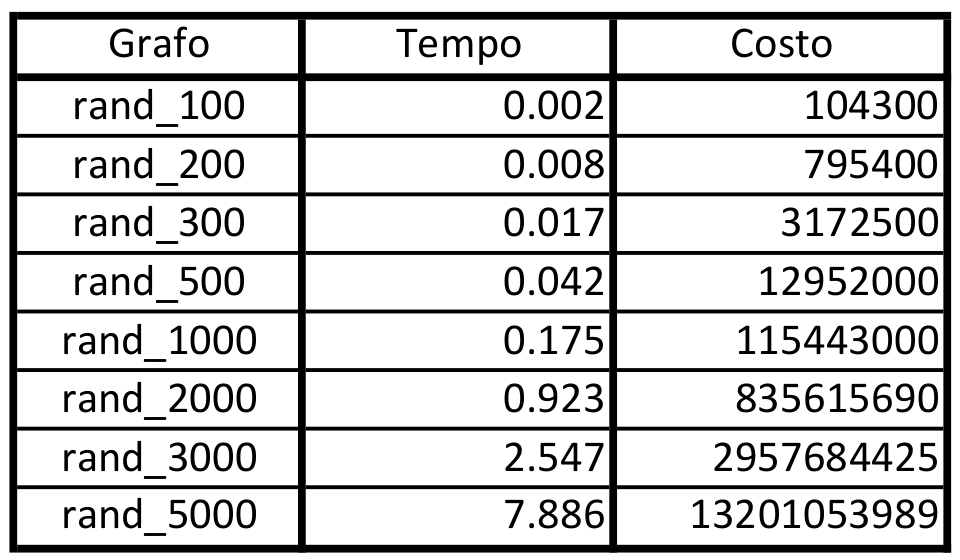
\includegraphics[width=200pt]{img/CHRrandom.png}
        \caption*{Su grafi generati casualmente.}
    \end{subfigure}
    \ \\
    \ \\
    \ \\
    \ \\
    \begin{subfigure}{\linewidth}
        \centering
        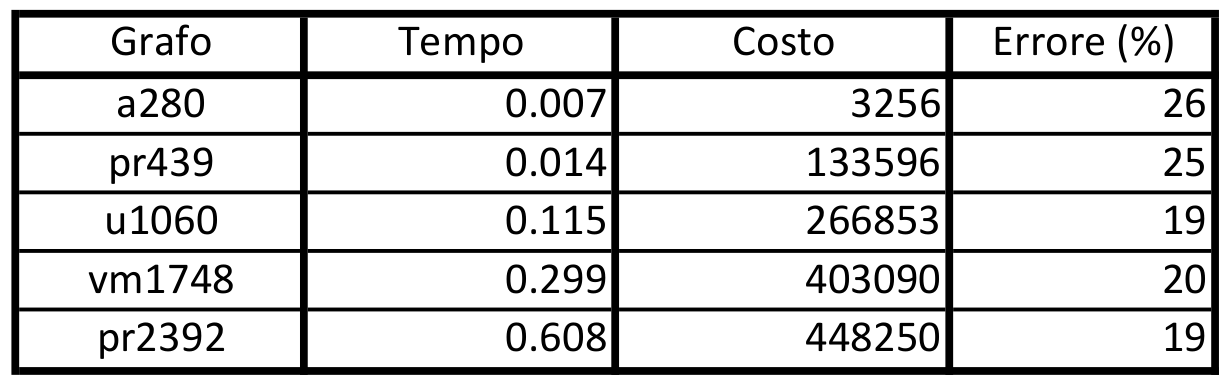
\includegraphics[width=300pt]{img/CHRtsplib.png}
        \caption*{Su grafi di \texttt{TSPLIB}.}
    \end{subfigure}
    \caption{Risultati \texttt{CHR}.}
\end{figure}
\ \\
\ \\

\begin{figure}[H]
    \centering
    \begin{subfigure}{\linewidth}
        \centering
        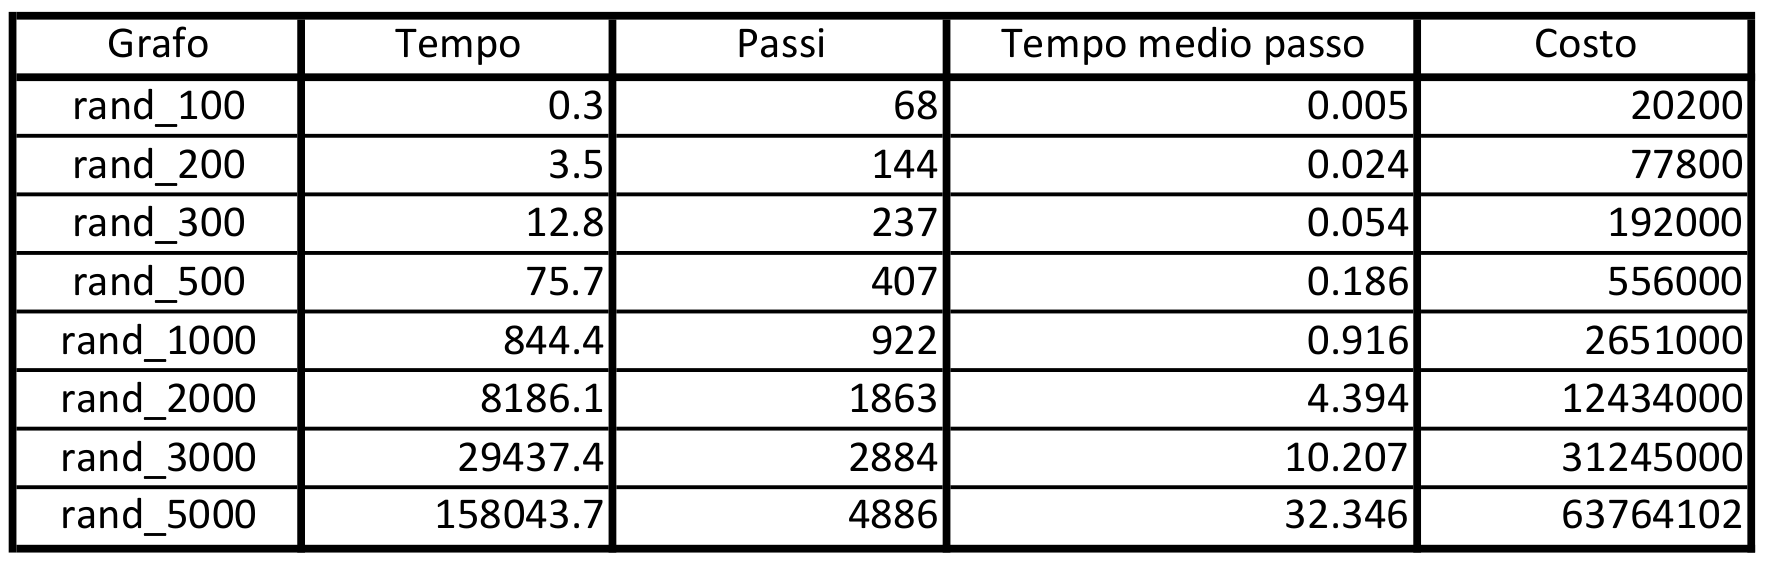
\includegraphics[width=400pt]{img/L3ORrandom.png}
        \caption*{Su grafi generati casualmente.}
    \end{subfigure}
    \ \\
    \ \\
    \ \\
    \ \\
    \begin{subfigure}{\linewidth}
        \centering
        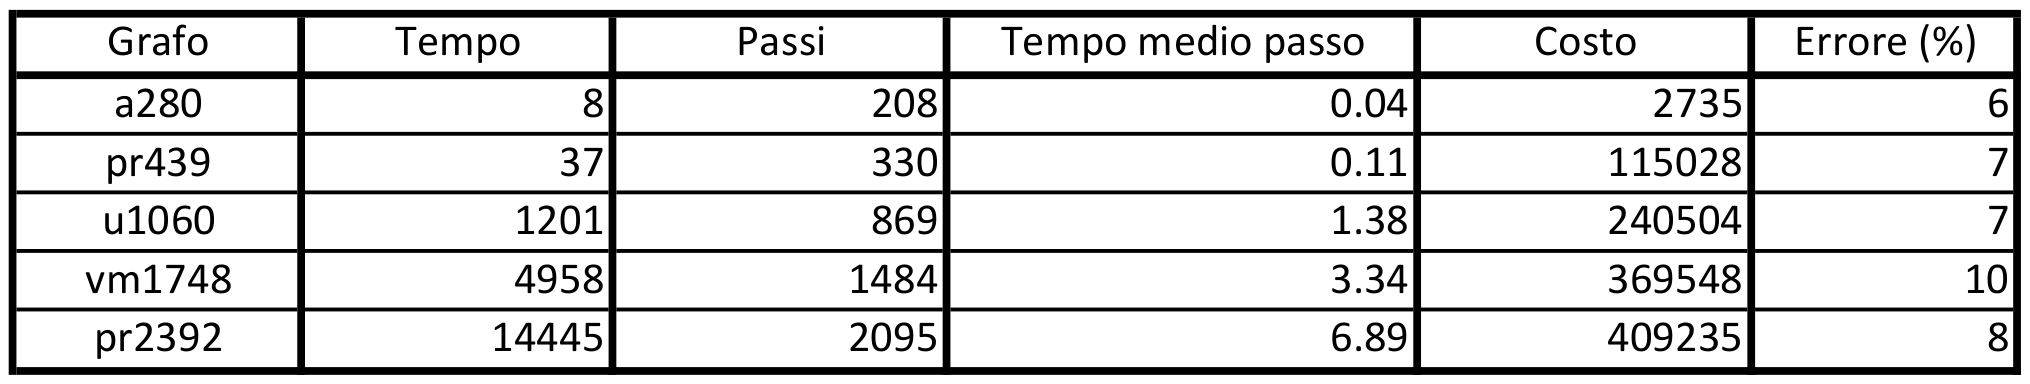
\includegraphics[width=400pt]{img/L3ORtsplib.png}
        \caption*{Su grafi di \texttt{TSPLIB}.}
    \end{subfigure}
    \caption{Risultati \texttt{L3OR}.}
\end{figure}
\ \\

\begin{figure}[H]
    \centering
    \begin{subfigure}{\linewidth}
        \centering
        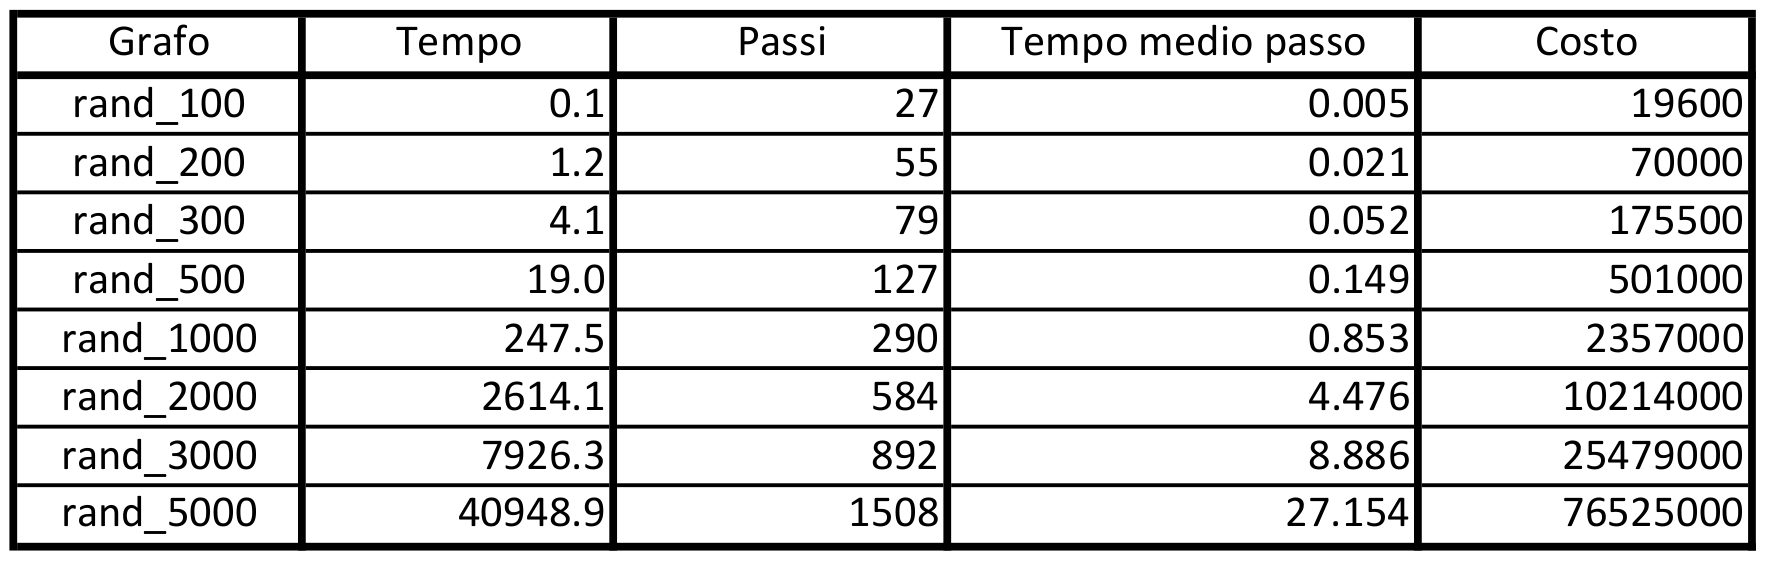
\includegraphics[width=400pt]{img/L3OCrandom.png}
        \caption*{Su grafi generati casualmente.}
    \end{subfigure}
    \ \\
    \ \\
    \ \\
    \ \\
    \begin{subfigure}{\linewidth}
        \centering
        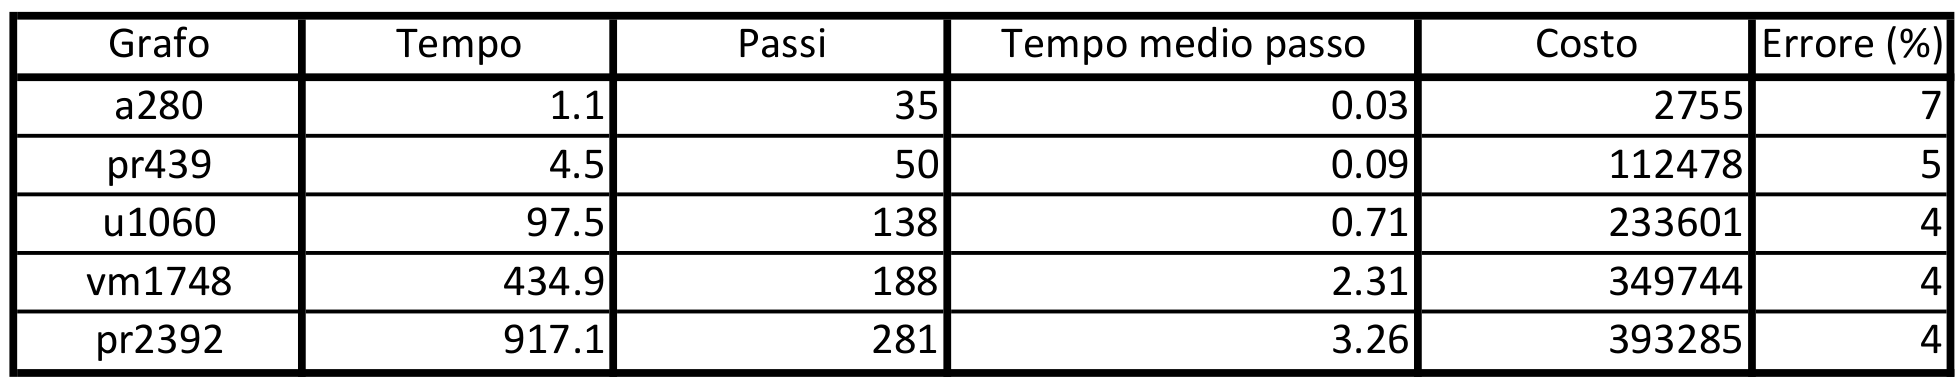
\includegraphics[width=400pt]{img/L3OCtsplib.png}
        \caption*{Su grafi di \texttt{TSPLIB}.}
    \end{subfigure}
    \caption{Risultati \texttt{L3OC}.}
\end{figure}
\ \\
\ \\

\begin{figure}[H]
    \centering
    \begin{subfigure}{\linewidth}
        \centering
        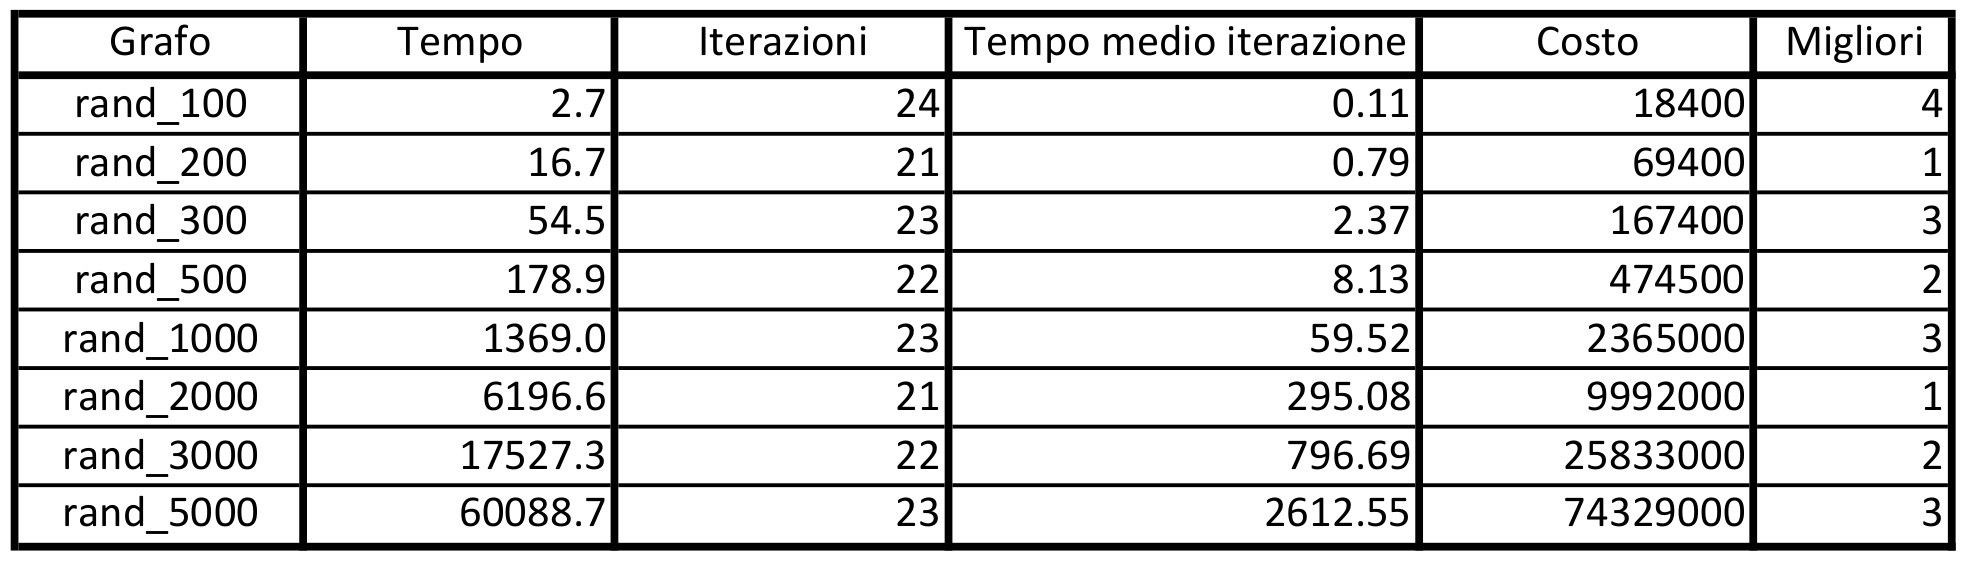
\includegraphics[width=400pt]{img/RL3Orandom.png}
        \caption*{Su grafi generati casualmente.}
    \end{subfigure}
    \ \\
    \ \\
    \ \\
    \ \\
    \begin{subfigure}{\linewidth}
        \centering
        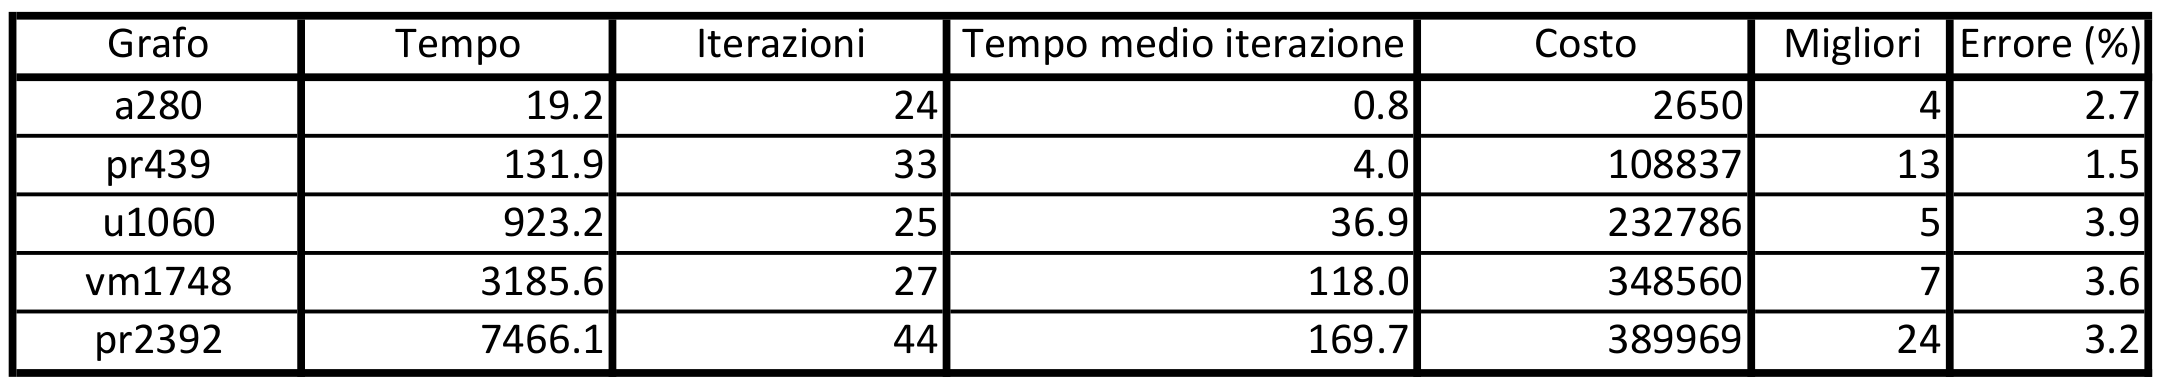
\includegraphics[width=400pt]{img/RL3Otsplib.png}
        \caption*{Su grafi di \texttt{TSPLIB}.}
    \end{subfigure}
    \ \\
    \ \\
    \ \\
    \ \\
    \begin{subfigure}{\linewidth}
        \centering
        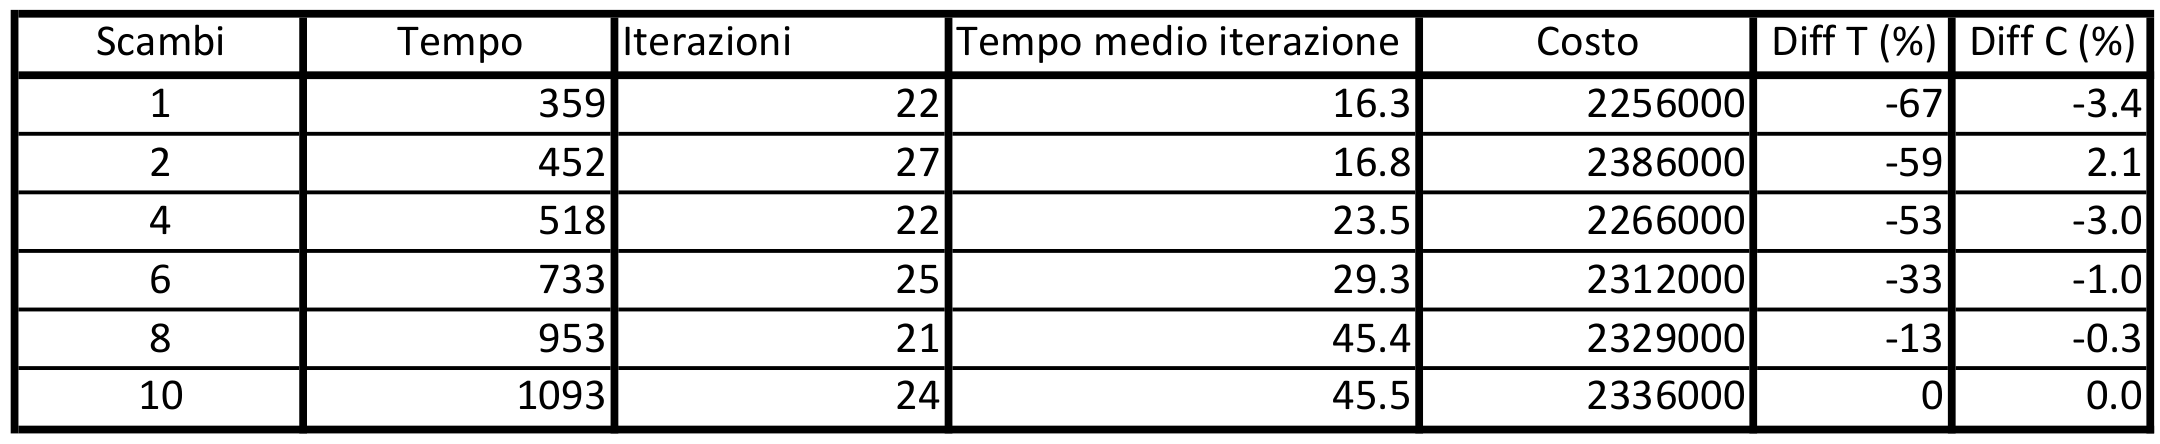
\includegraphics[width=400pt]{img/RL3Oscambi.png}
        \caption*{Su un campione di grafi causali di $n=1000$ nodi, al variare di \texttt{maxExchanges}.}
    \end{subfigure}
    \caption{Risultati \texttt{RL3O}.}
\end{figure}
\ \\
\ \\

\begin{figure}[H]
    \centering
    \begin{subfigure}{\linewidth}
        \centering
        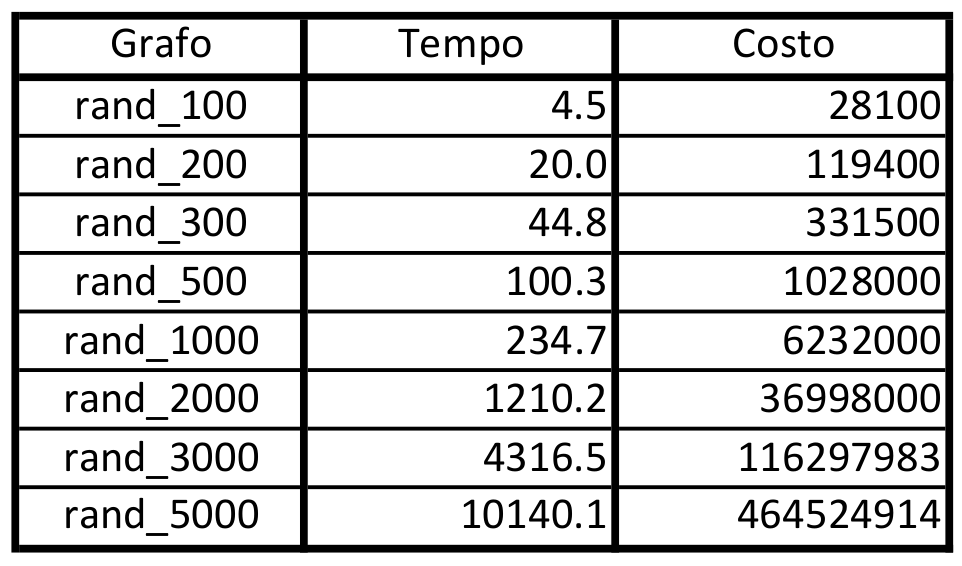
\includegraphics[width=200pt]{img/LKHrandom.png}
        \caption*{Su grafi generati casualmente.}
    \end{subfigure}
    \ \\
    \ \\
    \ \\
    \ \\
    \begin{subfigure}{\linewidth}
        \centering
        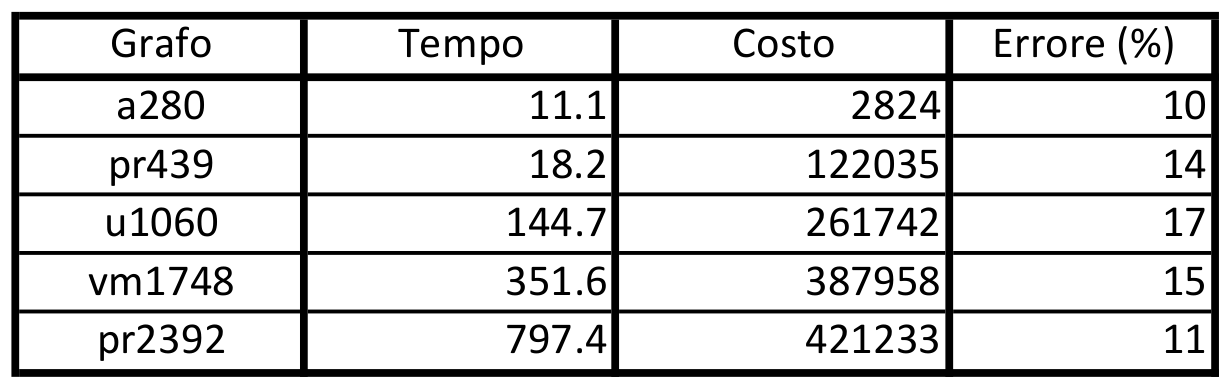
\includegraphics[width=300pt]{img/LKHtsplib.png}
        \caption*{Su grafi di \texttt{TSPLIB}.}
    \end{subfigure}
    \ \\
    \ \\
    \ \\
    \ \\
    \begin{subfigure}{\linewidth}
        \centering
        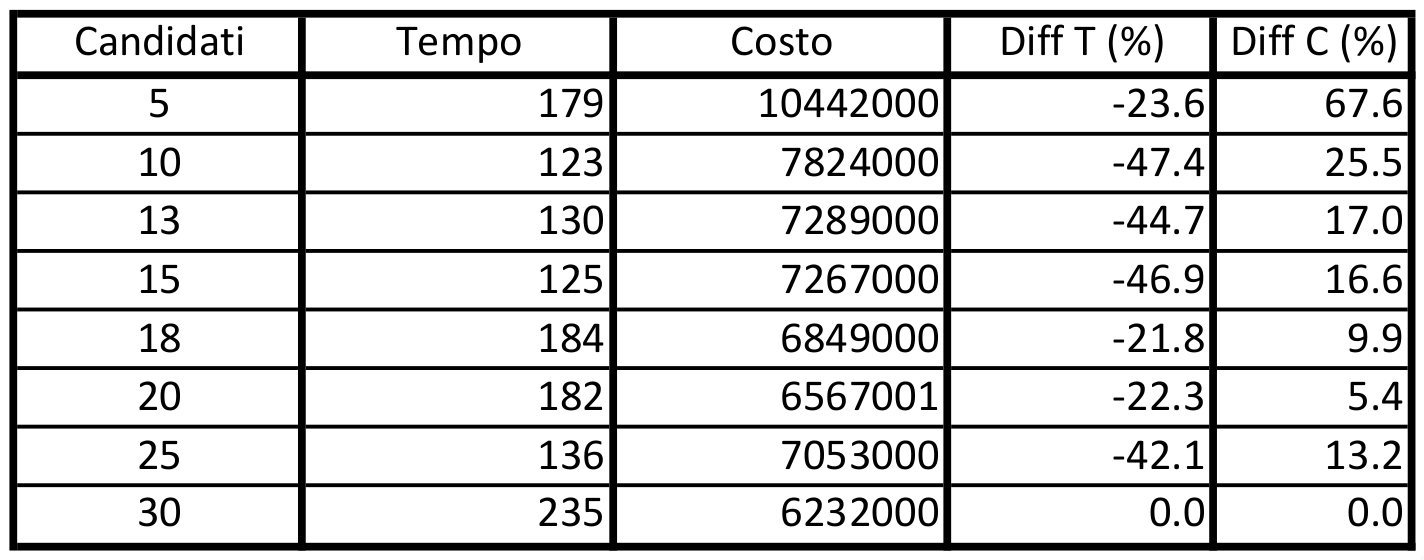
\includegraphics[width=300pt]{img/LKHcandidati.png}
        \caption*{Su un campione di grafi causali di $n=1000$ nodi, al variare di \texttt{maxCandidates}.}
    \end{subfigure}
    \caption{Risultati \texttt{LKH}.}
\end{figure}

\newpage
\subsection{Tabelle e grafici dei confronti}

Vengono ora confrontati e commentati i risultati ottenuti: tempi e costi tra diverse euristiche, confronto 
nel numero di scambi in \texttt{RL3O} e confronto nel numero di candidati in \texttt{LKH}.

\begin{figure}[H]
    \centering
    \begin{subfigure}{\linewidth}
        \centering
        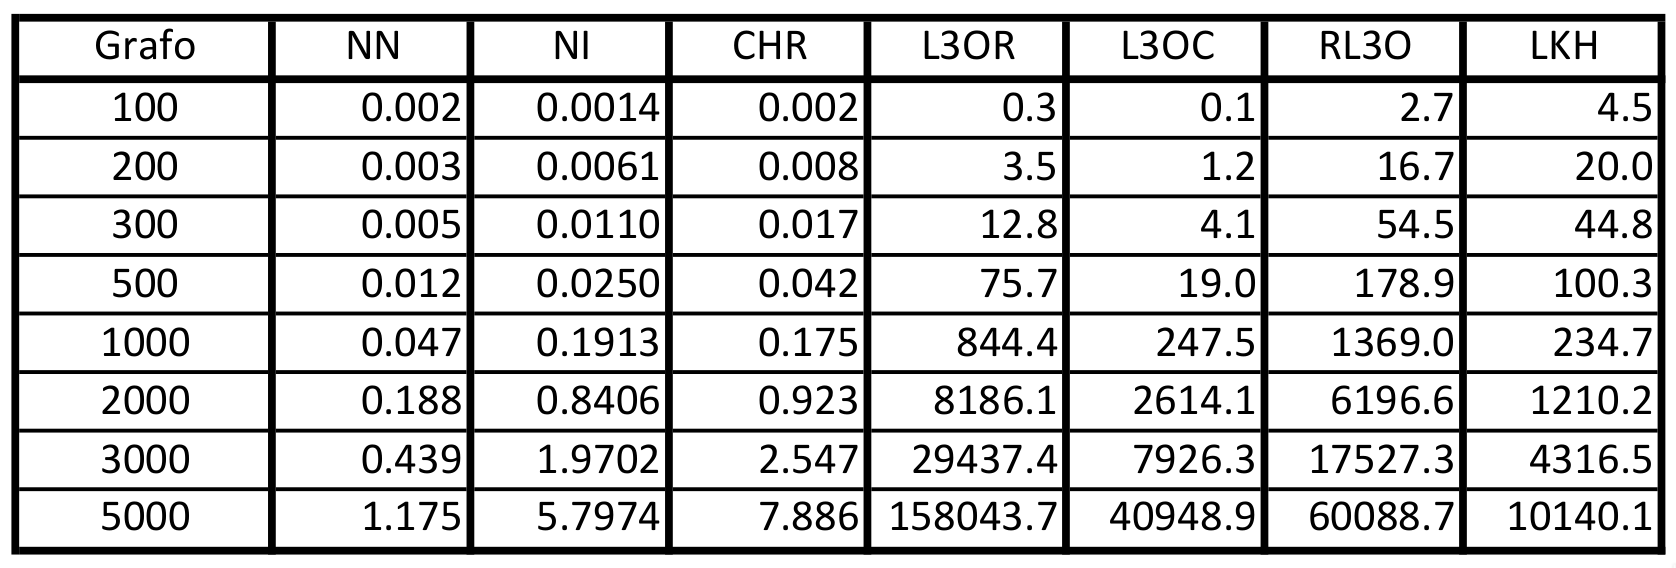
\includegraphics[width=320pt]{img/ConfrontoTempiRandom.png}
        \caption*{Su grafi generati casualmente.}
    \end{subfigure}
    \ \\
    \ \\
    \ \\
    \begin{subfigure}{\linewidth}
        \centering
        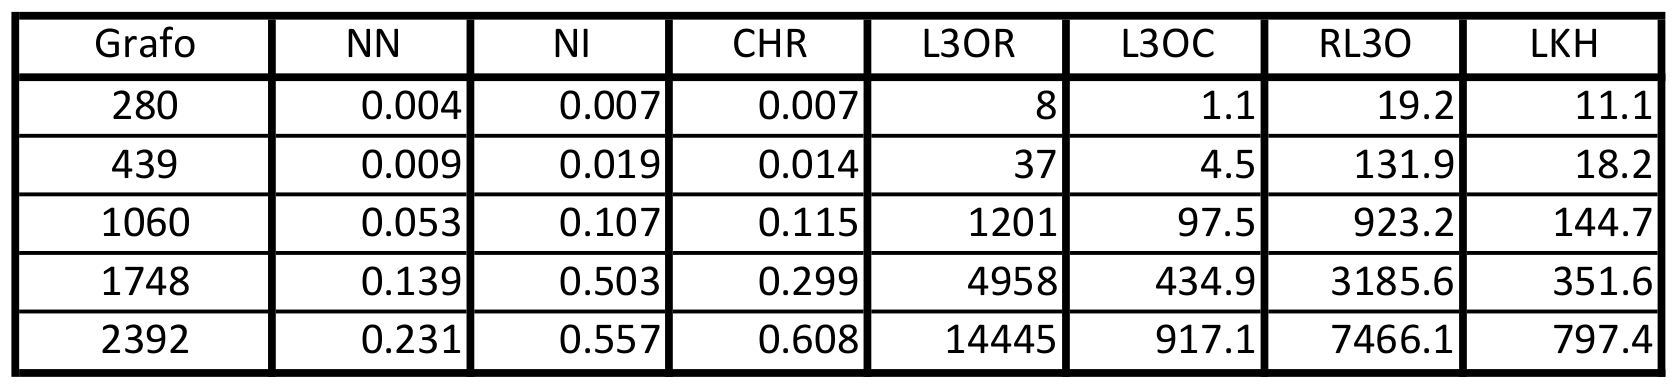
\includegraphics[width=320pt]{img/ConfrontoTempiTsplib.png}
        \caption*{Su grafi di \texttt{TSPLIB}.}
    \end{subfigure}
    \ \\
    \ \\
    \ \\
    \begin{subfigure}{\linewidth}
        \centering
        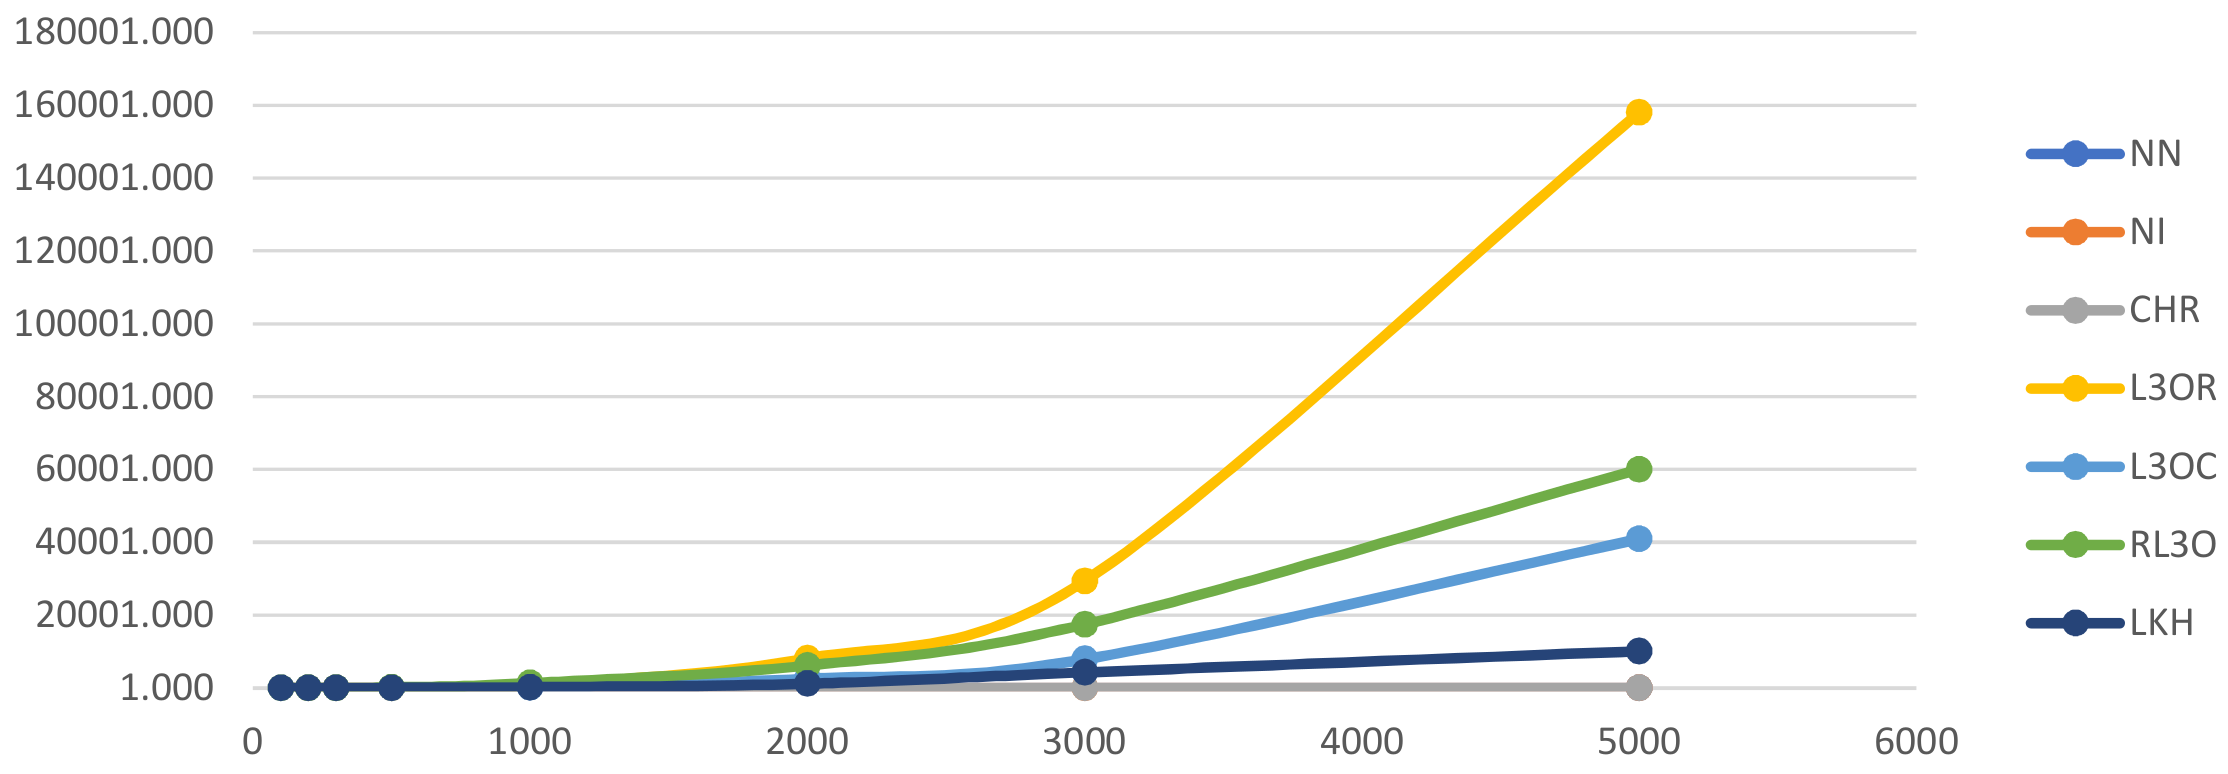
\includegraphics[width=300pt]{img/GraficoTempiRandom.png}
        \caption*{Su grafi generati casualmente.}
    \end{subfigure}
    \ \\
    \ \\
    \ \\
    \begin{subfigure}{\linewidth}
        \centering
        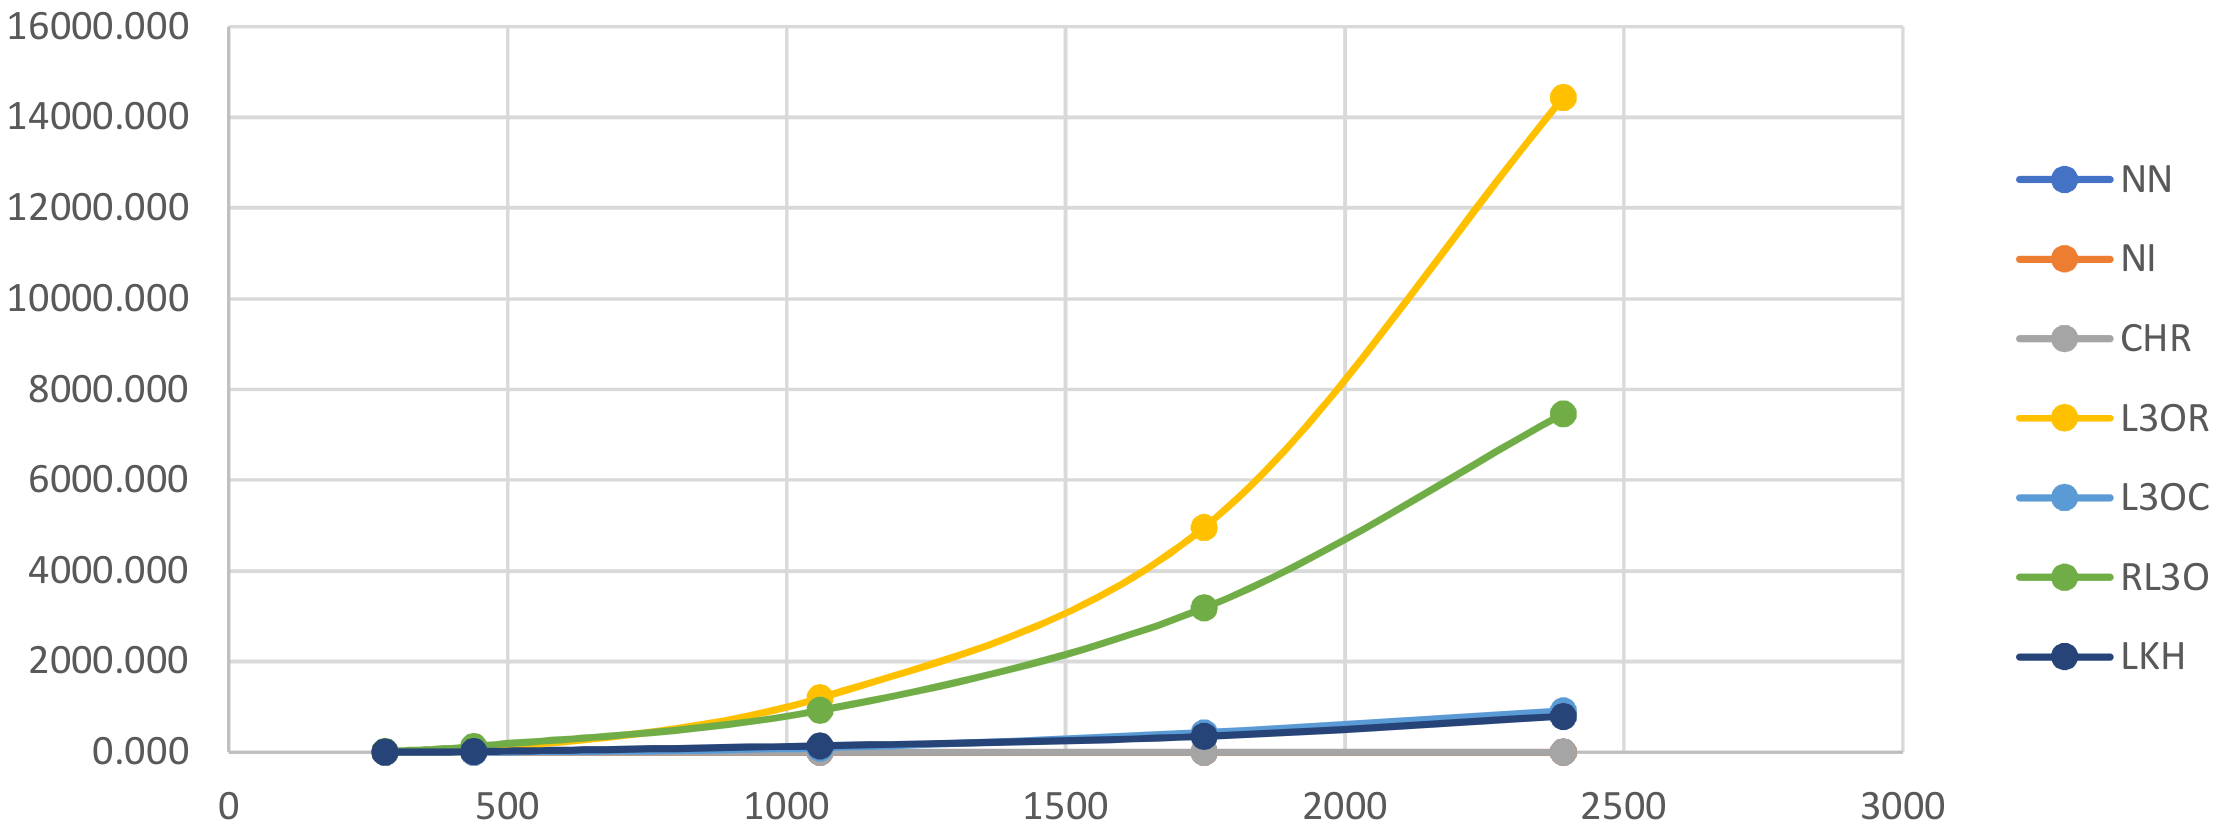
\includegraphics[width=300pt]{img/GraficoTempiTsplib.png}
        \caption*{Su grafi di \texttt{TSPLIB}.}
    \end{subfigure}
    \caption{Confronto diretto dei tempi di esecuzione delle diverse euristiche.}
\end{figure}

Da come si evince dai grafici, le euristiche ``tour construction'' sono le vincitrici per 
quanto riguarda la velocità di esecuzione; il più lento è \texttt{LR3O} con un notevole distacco (più del doppio 
del tempo rispetto al penultimo \texttt{RL3O}); \texttt{LKH} si dimostra sorprendemente veloce. Il trend si 
mantiene sia sui grafi casuali, sia sui grafi di \texttt{TSPLIB}.

\begin{figure}[H]
    \centering
    \begin{subfigure}{\linewidth}
        \centering
        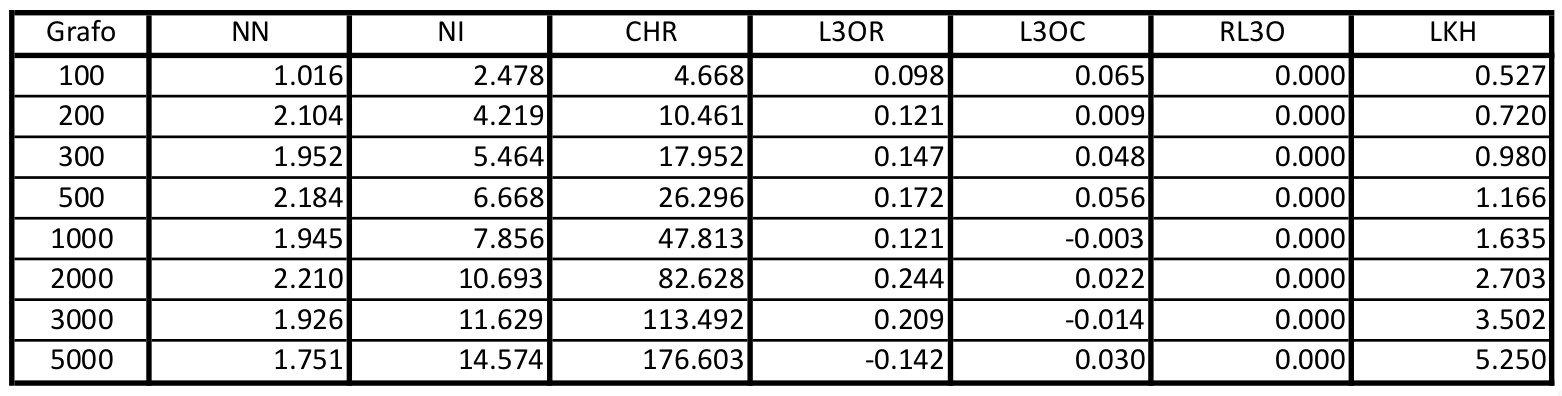
\includegraphics[width=350pt]{img/ConfrontoCostiRandom.png}
        \caption*{Su grafi generati casualmente.}
    \end{subfigure}
    \ \\
    \ \\
    \ \\
    \begin{subfigure}{\linewidth}
        \centering
        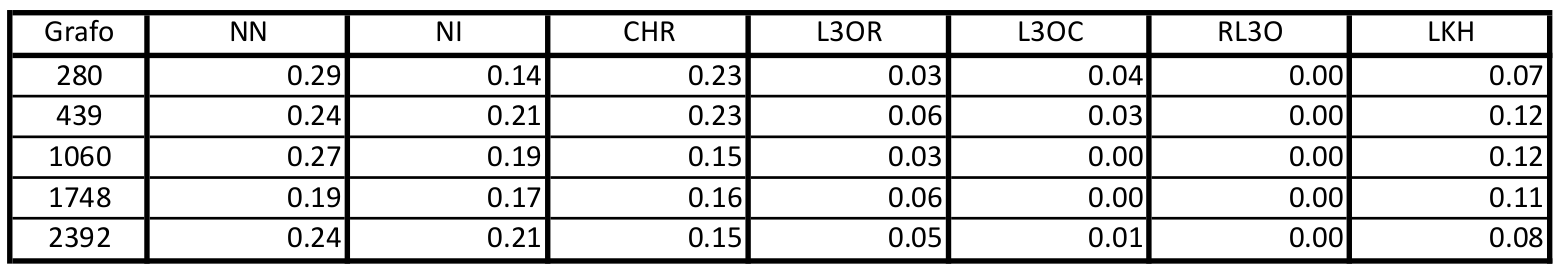
\includegraphics[width=350pt]{img/ConfrontoCostiTsplib.png}
        \caption*{Su grafi di \texttt{TSPLIB}.}
    \end{subfigure}
    \ \\
    \ \\
    \ \\
    \begin{subfigure}{\linewidth}
        \centering
        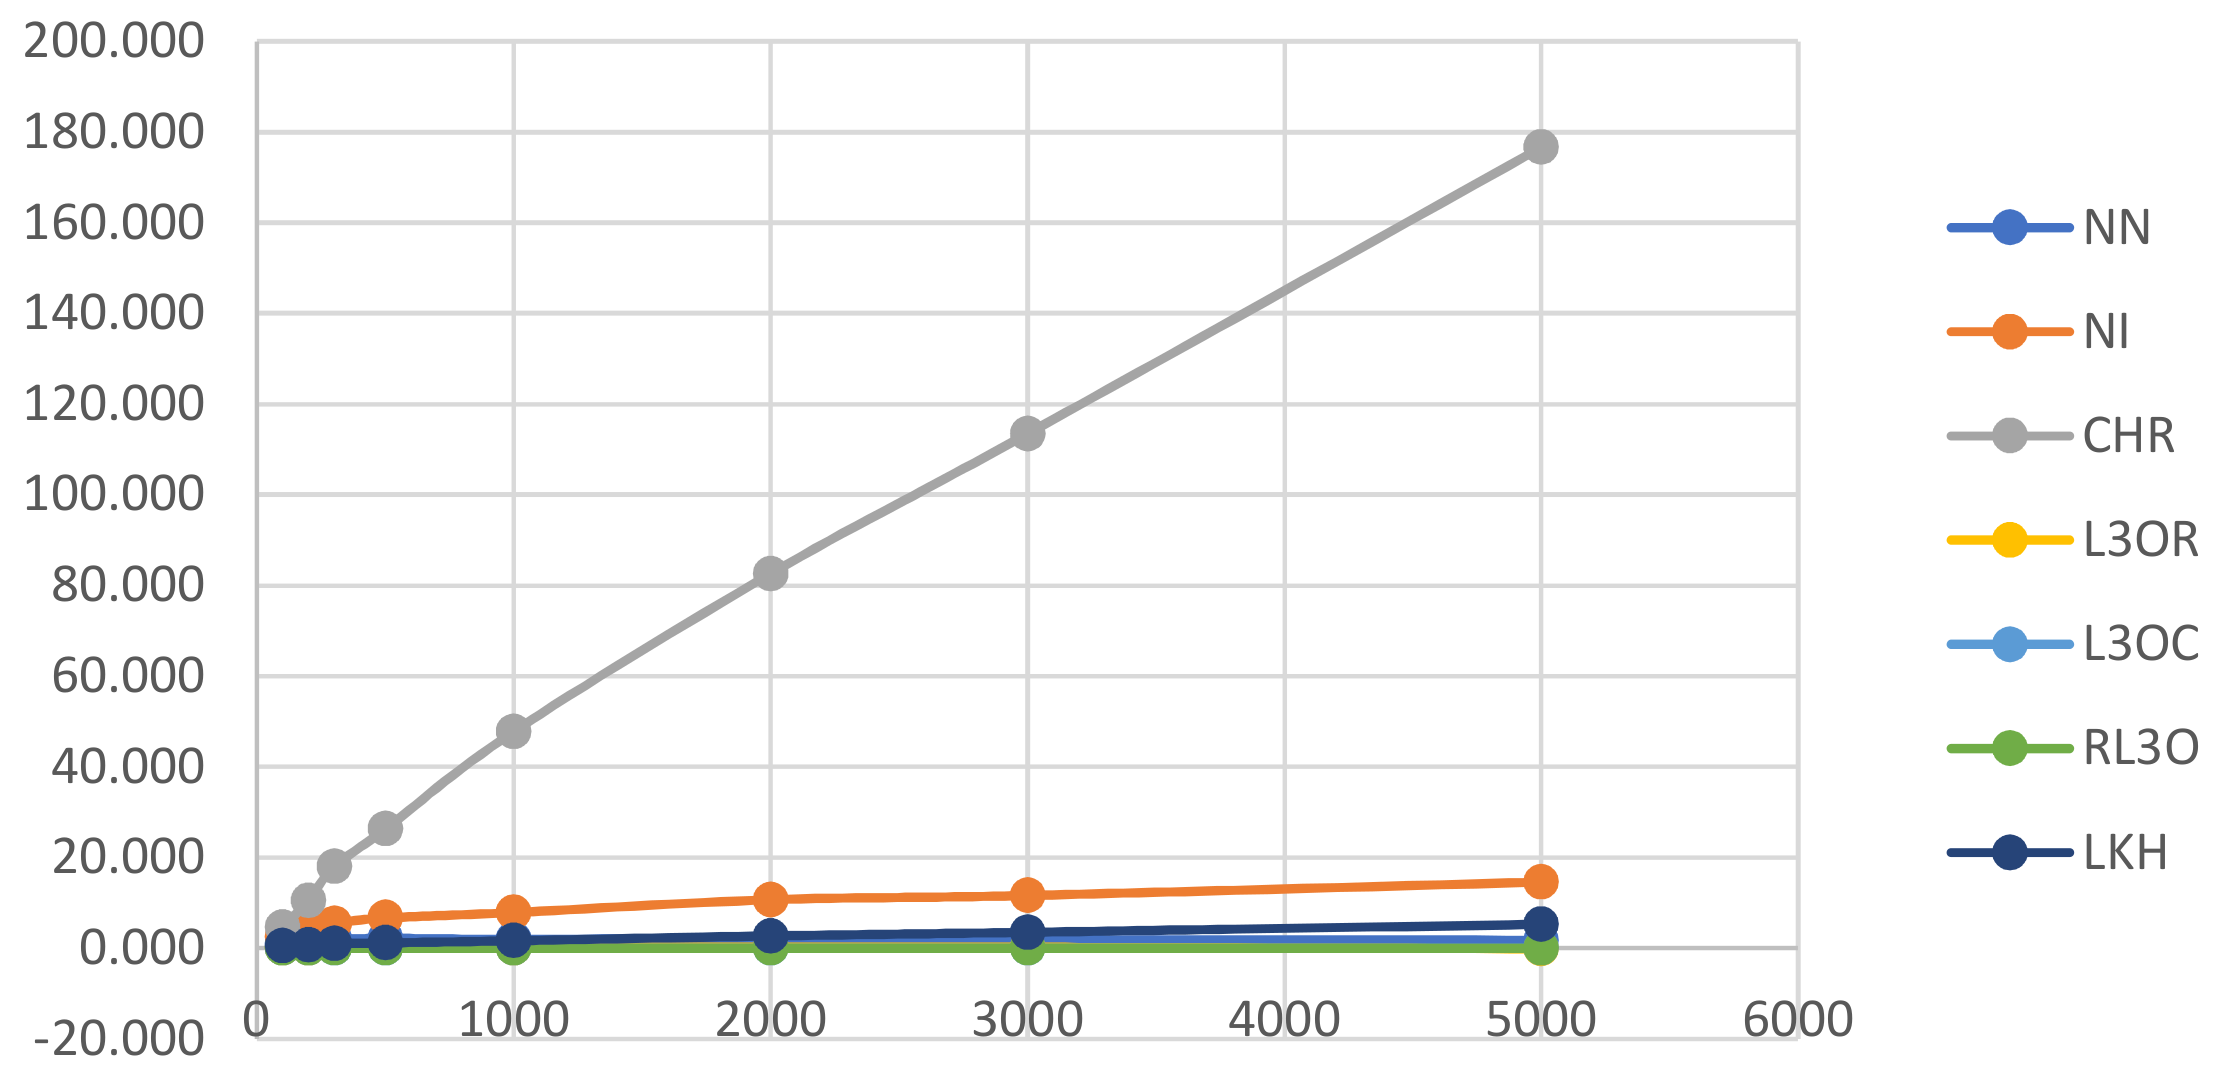
\includegraphics[width=270pt]{img/GraficoCostiRandomConCHR.png}
        \caption*{Su grafi generati casualmente, con la presenza di \texttt{CHR}.}
    \end{subfigure}
    \ \\
    \ \\
    \ \\
    \begin{subfigure}{\linewidth}
        \centering
        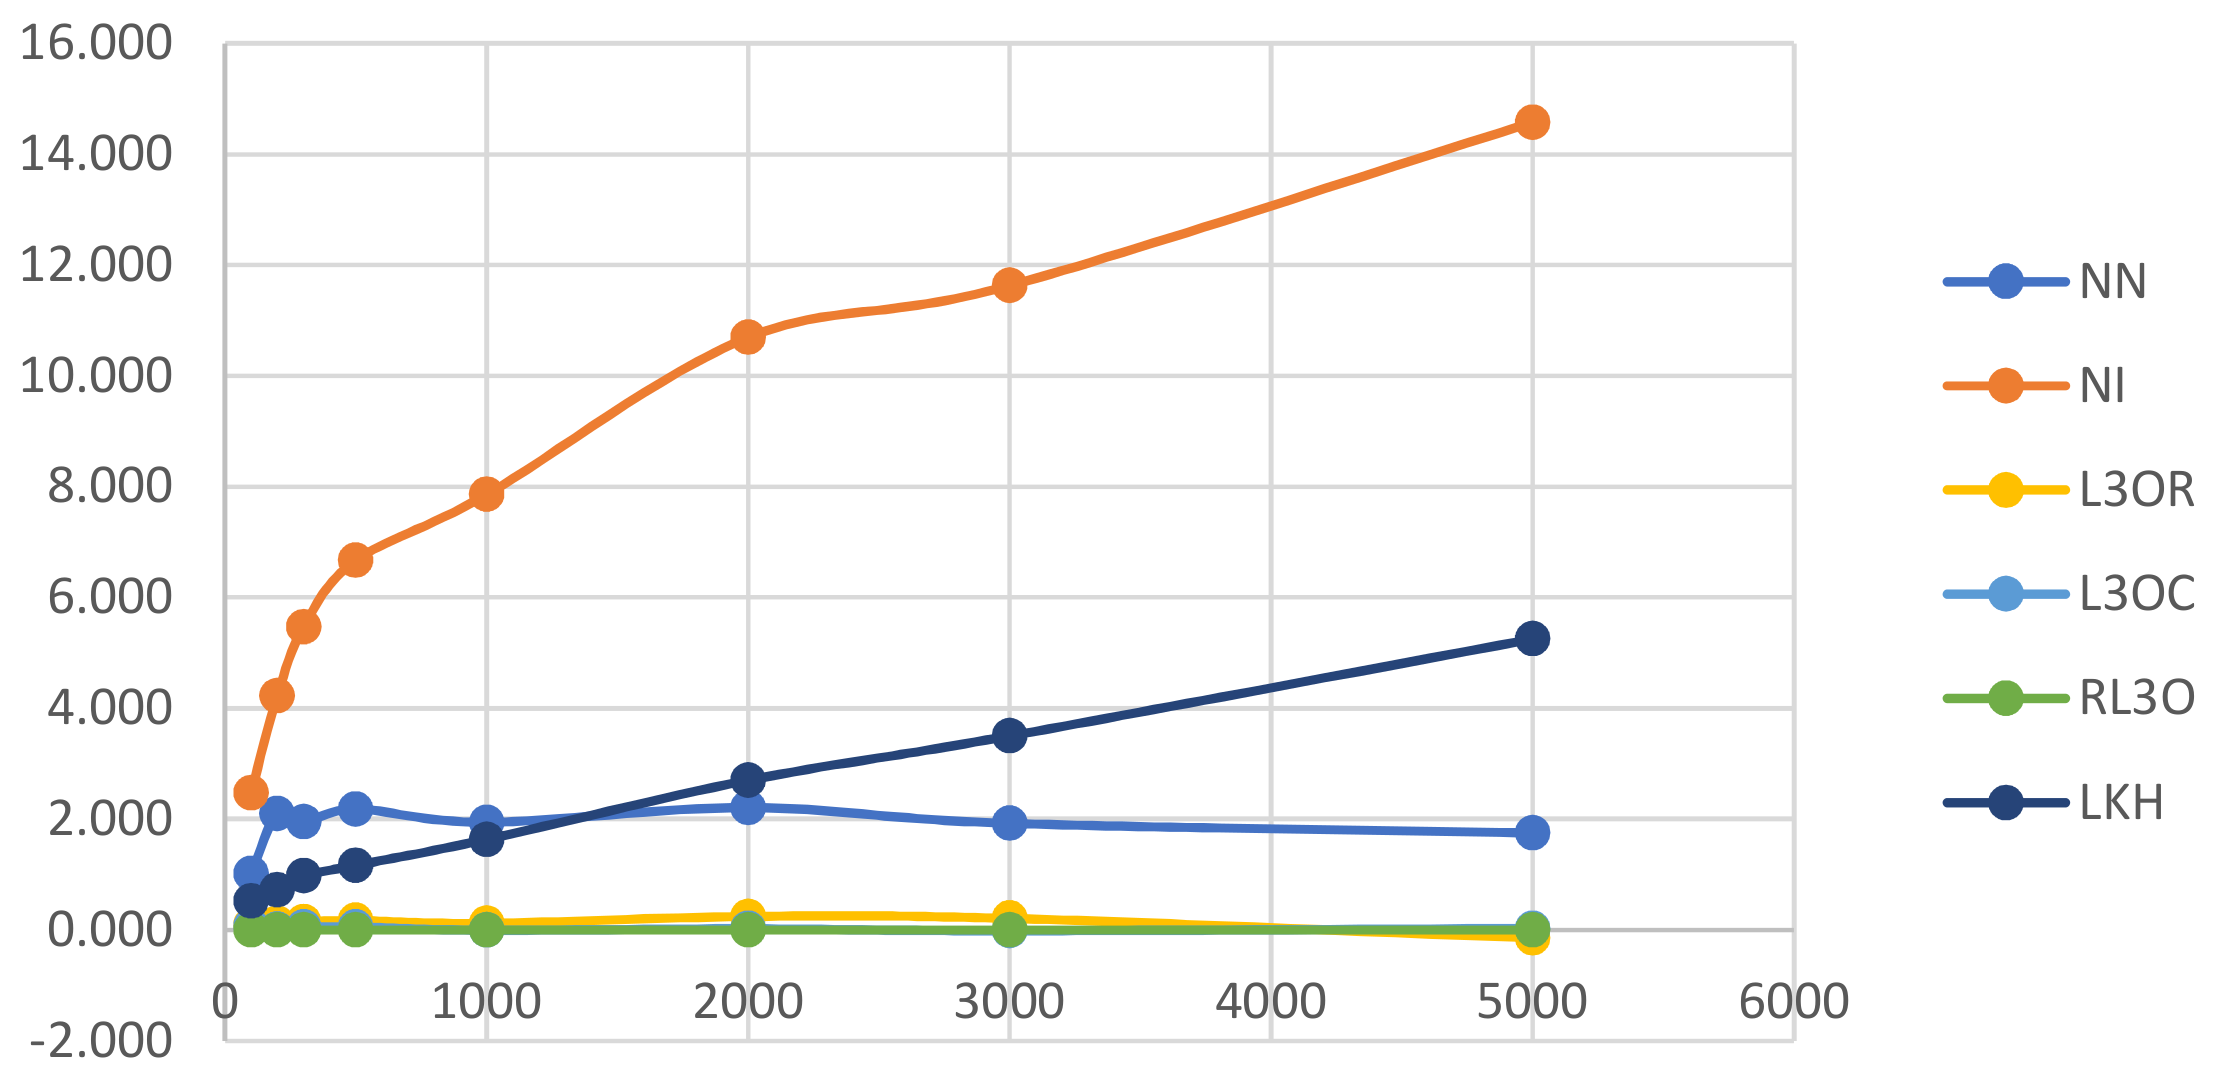
\includegraphics[width=270pt]{img/GraficoCostiRandomSenzaCHR.png}
        \caption*{Su grafi generati casualmente, senza \texttt{CHR} (che ha trovato tour 
                    molto più costosi).}
    \end{subfigure}
    \ \\
    \ \\
    \ \\
    \begin{subfigure}{\linewidth}
        \centering
        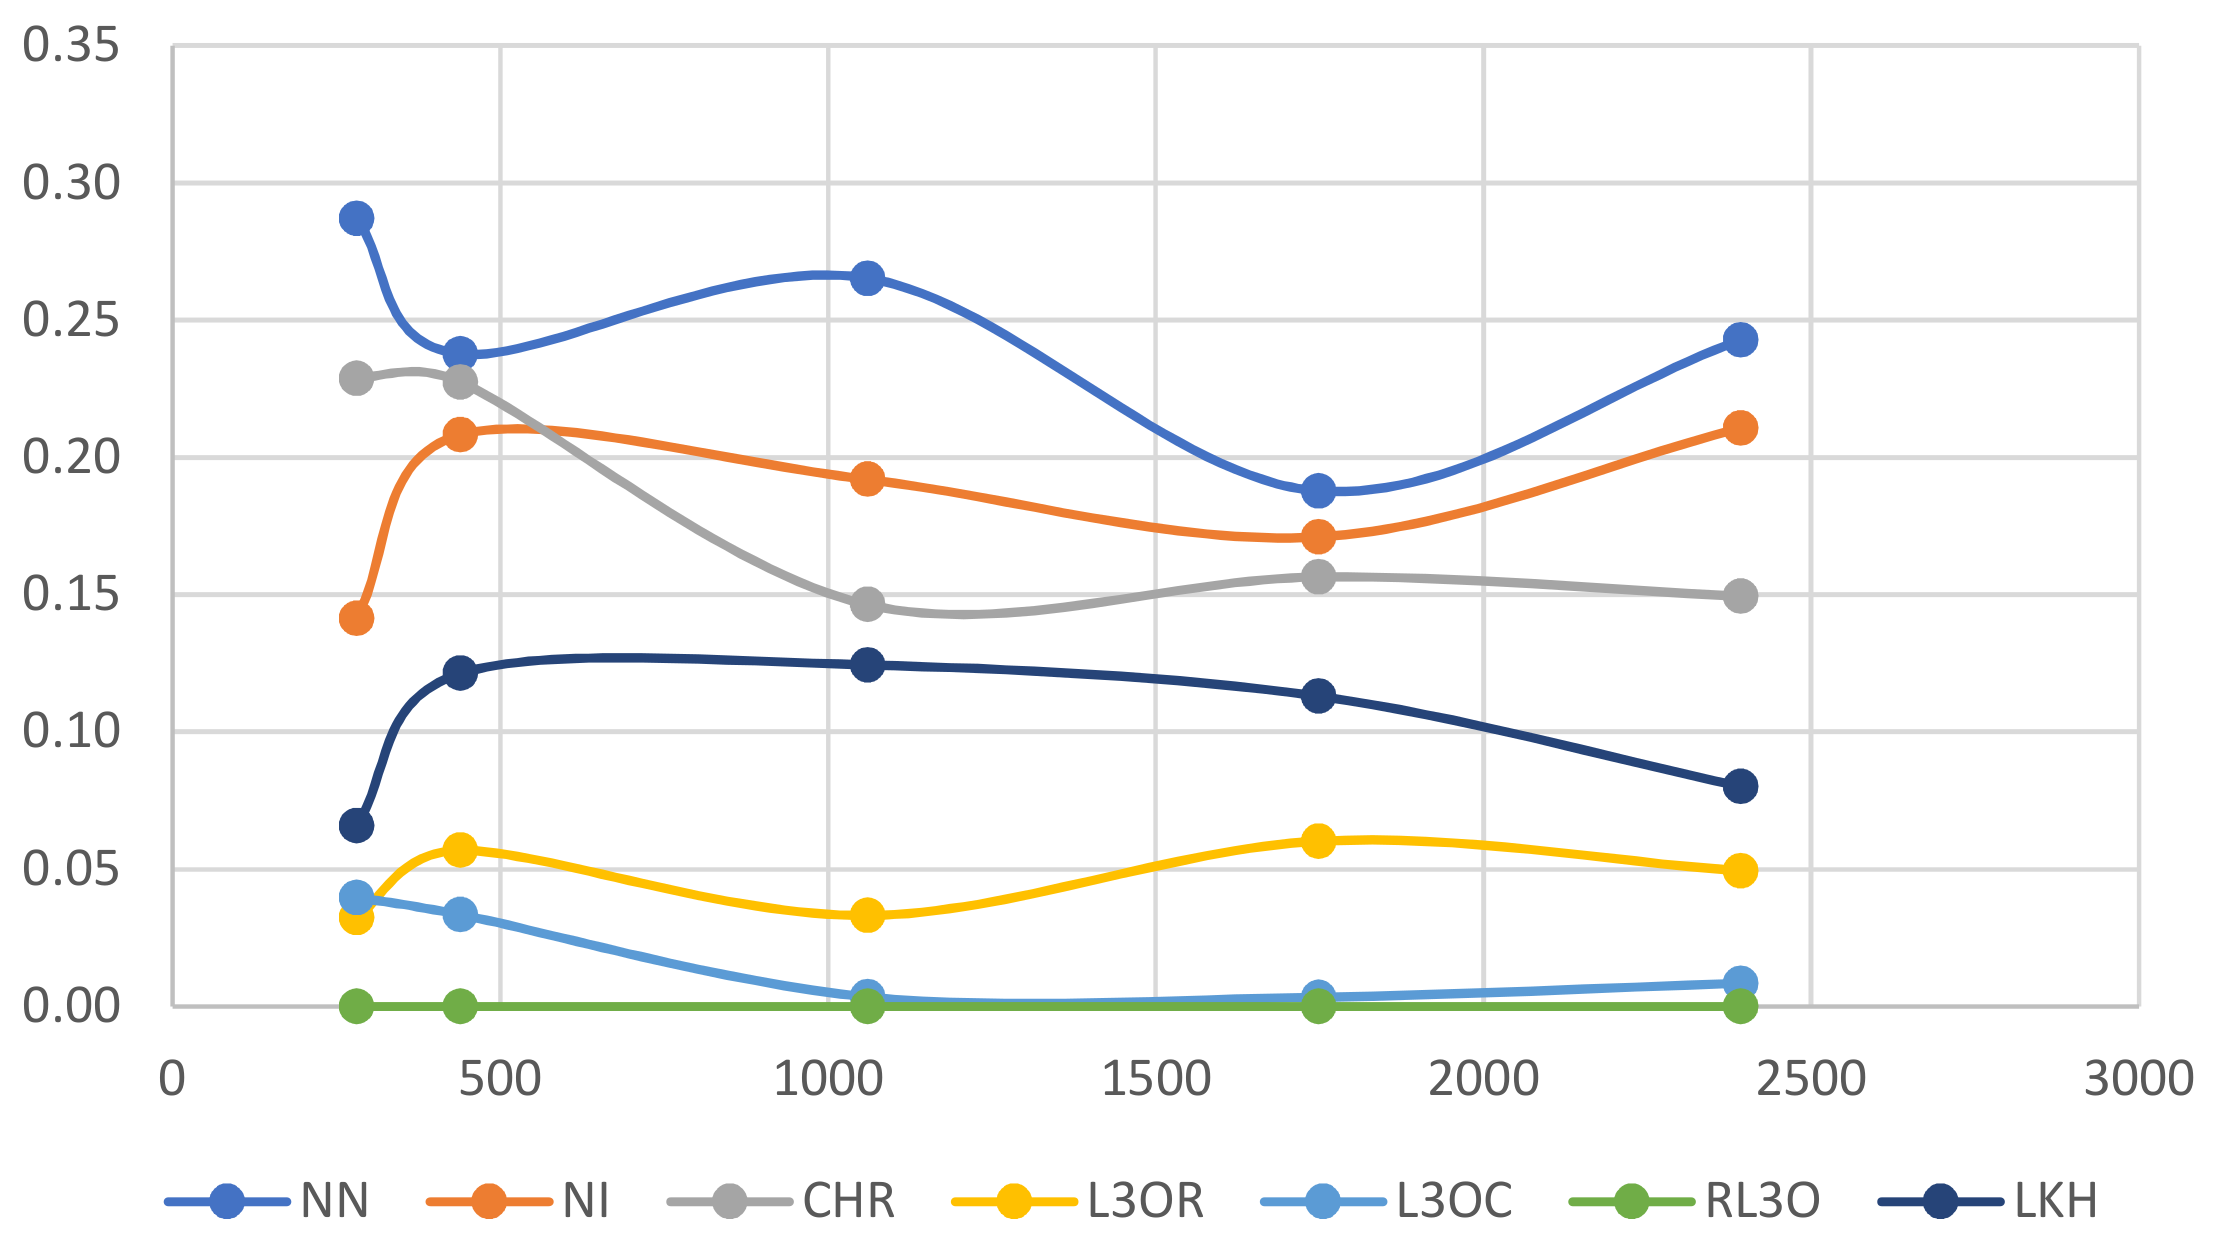
\includegraphics[width=270pt]{img/GraficoCostiTsplib.png}
        \caption*{Su grafi di \texttt{TSPLIB}.}
    \end{subfigure}
    \caption{Confronto diretto dei costi dei tour trovati dalle diverse euristiche.}
\end{figure}

Situazione diametralmente opposta per quanto riguarda i costi: \texttt{L3OR} e \texttt{RL3O} 
si dimostrano i più precisi; \texttt{CHR} decisamente impreciso per quanto riguarda i grafi 
casuali, tanto da rendere necessaria la visualizzazione grafica dei dati senza la sua presenza.
Per quanto riguarda i grafi di \texttt{TSPLIB} la situazione è più equilibrata. I confronti sui 
costi, non essendo noti gli ottimi di una delle classi di grafi, sono stati fatti in differenza 
percentuale rispetto a \texttt{RL3O}.
\ \\
\ \\

\begin{figure}[H]
    \centering
    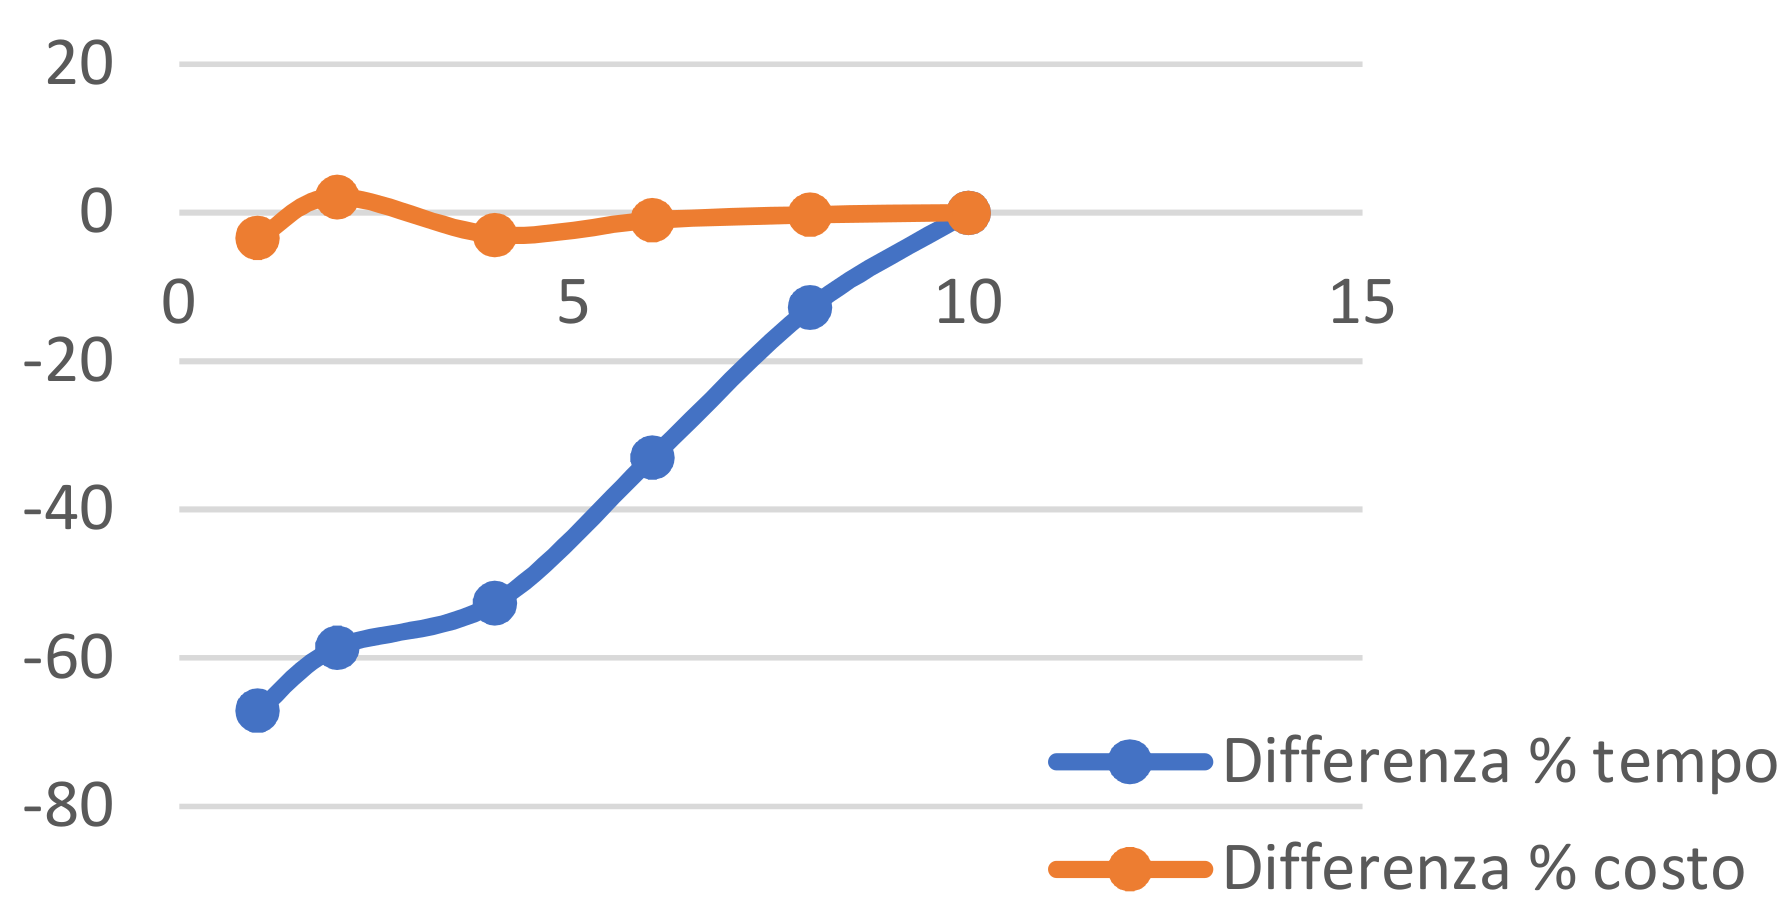
\includegraphics[width=250pt]{img/GraficoScambi.png}
    \caption{Confronto tra efficienza ed efficacia di \texttt{RL3O} al variare del numero massimo 
                di \textit{exchanges}.}
\end{figure}

Per quanto riguarda la scelta del numero massimo di scambi sembra non esserci una differenza 
sostanziale nei costi dei tour trovati quando tali scambi sono contenuti. Prevedibile, invece, 
il guadagno in tempo se riduciamo il numero di scambi: meno scambi significa, intuitivamente, che 
il tour è molto simile a prima e quindi richiede meno passi \textit{best-improving} per riottenere 
il minimo locale.
\ \\
\ \\

\begin{figure}[H]
    \centering
    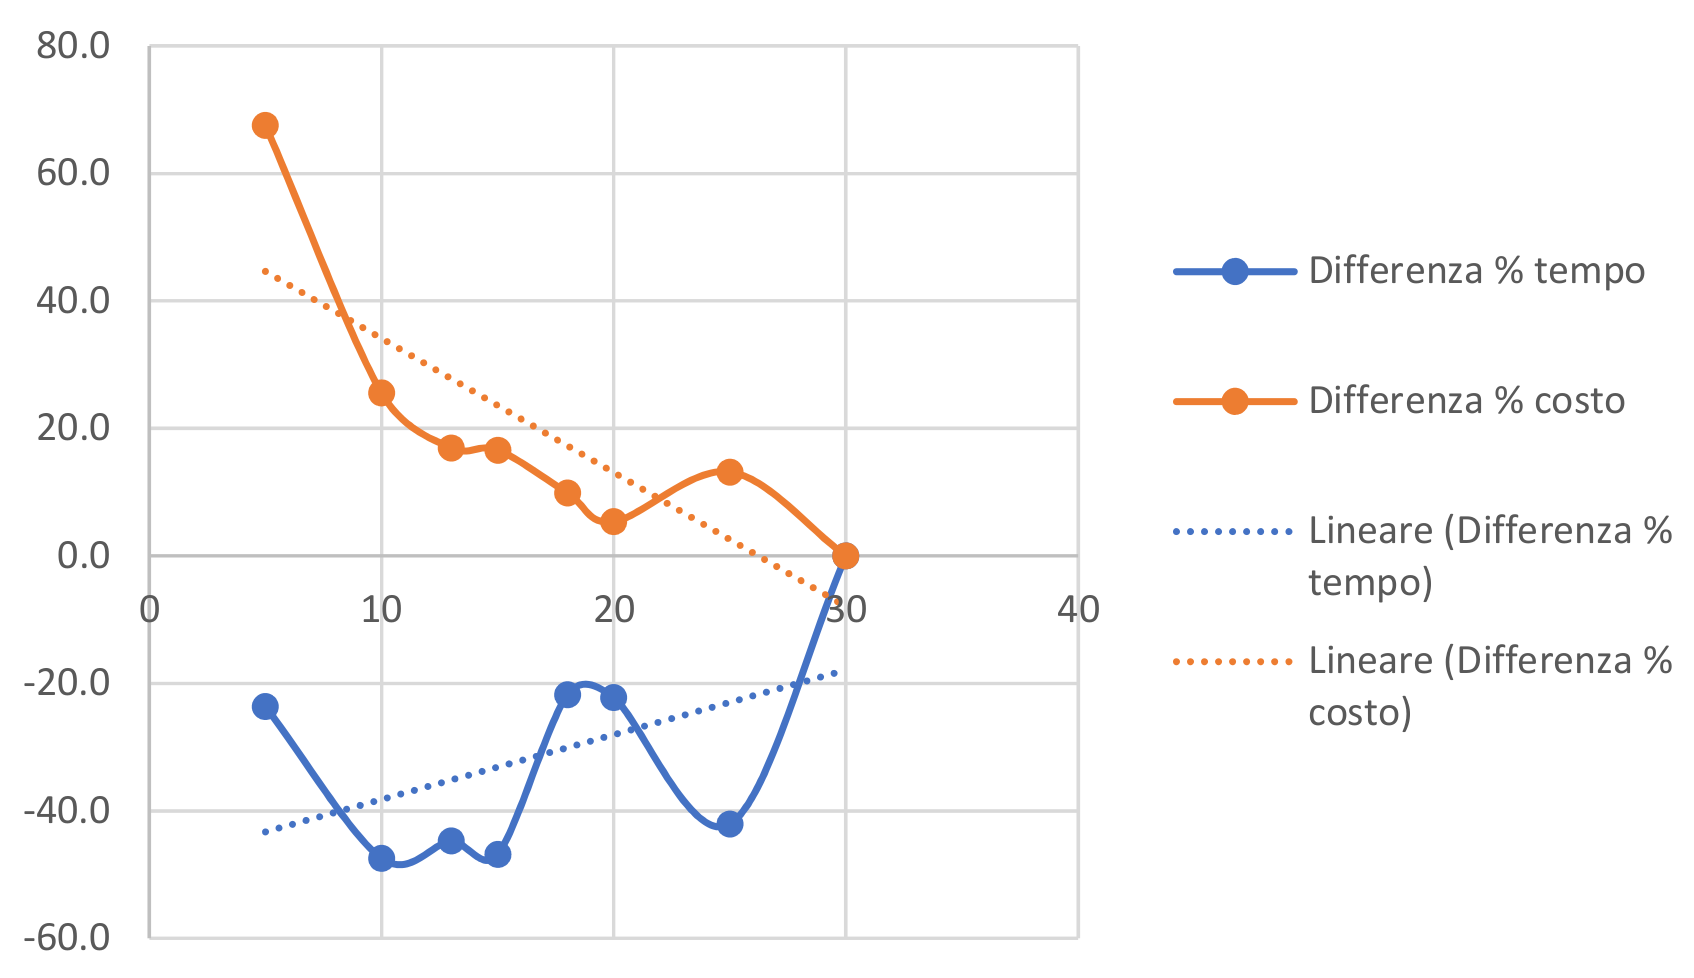
\includegraphics[width=300pt]{img/GraficoCandidati.png}
    \caption{Confronto tra efficienza ed efficacia di \texttt{LKH} al variare del numero massimo 
                di candidati per ogni \textit{candidate set}.}
\end{figure}

Prevedibile anche il risultato del test sul numero di candidati: la tendenza è quella di trovare 
tour più costosi e in meno tempo se i candidati sono pochi e tour meno costosi ma in più tempo 
se i candidati sono di più. Questo è anche il comportamento che ci si aspetterebbe da 
un'euristica, ovvero il tradeoff qualità/tempo.